% Options for packages loaded elsewhere
\PassOptionsToPackage{unicode}{hyperref}
\PassOptionsToPackage{hyphens}{url}
%
\documentclass[
]{article}
\usepackage{amsmath,amssymb}
\usepackage{lmodern}
\usepackage{iftex}
\ifPDFTeX
  \usepackage[T1]{fontenc}
  \usepackage[utf8]{inputenc}
  \usepackage{textcomp} % provide euro and other symbols
\else % if luatex or xetex
  \usepackage{unicode-math}
  \defaultfontfeatures{Scale=MatchLowercase}
  \defaultfontfeatures[\rmfamily]{Ligatures=TeX,Scale=1}
\fi
% Use upquote if available, for straight quotes in verbatim environments
\IfFileExists{upquote.sty}{\usepackage{upquote}}{}
\IfFileExists{microtype.sty}{% use microtype if available
  \usepackage[]{microtype}
  \UseMicrotypeSet[protrusion]{basicmath} % disable protrusion for tt fonts
}{}
\makeatletter
\@ifundefined{KOMAClassName}{% if non-KOMA class
  \IfFileExists{parskip.sty}{%
    \usepackage{parskip}
  }{% else
    \setlength{\parindent}{0pt}
    \setlength{\parskip}{6pt plus 2pt minus 1pt}}
}{% if KOMA class
  \KOMAoptions{parskip=half}}
\makeatother
\usepackage{xcolor}
\usepackage[margin=1in]{geometry}
\usepackage{color}
\usepackage{fancyvrb}
\newcommand{\VerbBar}{|}
\newcommand{\VERB}{\Verb[commandchars=\\\{\}]}
\DefineVerbatimEnvironment{Highlighting}{Verbatim}{commandchars=\\\{\}}
% Add ',fontsize=\small' for more characters per line
\usepackage{framed}
\definecolor{shadecolor}{RGB}{248,248,248}
\newenvironment{Shaded}{\begin{snugshade}}{\end{snugshade}}
\newcommand{\AlertTok}[1]{\textcolor[rgb]{0.94,0.16,0.16}{#1}}
\newcommand{\AnnotationTok}[1]{\textcolor[rgb]{0.56,0.35,0.01}{\textbf{\textit{#1}}}}
\newcommand{\AttributeTok}[1]{\textcolor[rgb]{0.77,0.63,0.00}{#1}}
\newcommand{\BaseNTok}[1]{\textcolor[rgb]{0.00,0.00,0.81}{#1}}
\newcommand{\BuiltInTok}[1]{#1}
\newcommand{\CharTok}[1]{\textcolor[rgb]{0.31,0.60,0.02}{#1}}
\newcommand{\CommentTok}[1]{\textcolor[rgb]{0.56,0.35,0.01}{\textit{#1}}}
\newcommand{\CommentVarTok}[1]{\textcolor[rgb]{0.56,0.35,0.01}{\textbf{\textit{#1}}}}
\newcommand{\ConstantTok}[1]{\textcolor[rgb]{0.00,0.00,0.00}{#1}}
\newcommand{\ControlFlowTok}[1]{\textcolor[rgb]{0.13,0.29,0.53}{\textbf{#1}}}
\newcommand{\DataTypeTok}[1]{\textcolor[rgb]{0.13,0.29,0.53}{#1}}
\newcommand{\DecValTok}[1]{\textcolor[rgb]{0.00,0.00,0.81}{#1}}
\newcommand{\DocumentationTok}[1]{\textcolor[rgb]{0.56,0.35,0.01}{\textbf{\textit{#1}}}}
\newcommand{\ErrorTok}[1]{\textcolor[rgb]{0.64,0.00,0.00}{\textbf{#1}}}
\newcommand{\ExtensionTok}[1]{#1}
\newcommand{\FloatTok}[1]{\textcolor[rgb]{0.00,0.00,0.81}{#1}}
\newcommand{\FunctionTok}[1]{\textcolor[rgb]{0.00,0.00,0.00}{#1}}
\newcommand{\ImportTok}[1]{#1}
\newcommand{\InformationTok}[1]{\textcolor[rgb]{0.56,0.35,0.01}{\textbf{\textit{#1}}}}
\newcommand{\KeywordTok}[1]{\textcolor[rgb]{0.13,0.29,0.53}{\textbf{#1}}}
\newcommand{\NormalTok}[1]{#1}
\newcommand{\OperatorTok}[1]{\textcolor[rgb]{0.81,0.36,0.00}{\textbf{#1}}}
\newcommand{\OtherTok}[1]{\textcolor[rgb]{0.56,0.35,0.01}{#1}}
\newcommand{\PreprocessorTok}[1]{\textcolor[rgb]{0.56,0.35,0.01}{\textit{#1}}}
\newcommand{\RegionMarkerTok}[1]{#1}
\newcommand{\SpecialCharTok}[1]{\textcolor[rgb]{0.00,0.00,0.00}{#1}}
\newcommand{\SpecialStringTok}[1]{\textcolor[rgb]{0.31,0.60,0.02}{#1}}
\newcommand{\StringTok}[1]{\textcolor[rgb]{0.31,0.60,0.02}{#1}}
\newcommand{\VariableTok}[1]{\textcolor[rgb]{0.00,0.00,0.00}{#1}}
\newcommand{\VerbatimStringTok}[1]{\textcolor[rgb]{0.31,0.60,0.02}{#1}}
\newcommand{\WarningTok}[1]{\textcolor[rgb]{0.56,0.35,0.01}{\textbf{\textit{#1}}}}
\usepackage{graphicx}
\makeatletter
\def\maxwidth{\ifdim\Gin@nat@width>\linewidth\linewidth\else\Gin@nat@width\fi}
\def\maxheight{\ifdim\Gin@nat@height>\textheight\textheight\else\Gin@nat@height\fi}
\makeatother
% Scale images if necessary, so that they will not overflow the page
% margins by default, and it is still possible to overwrite the defaults
% using explicit options in \includegraphics[width, height, ...]{}
\setkeys{Gin}{width=\maxwidth,height=\maxheight,keepaspectratio}
% Set default figure placement to htbp
\makeatletter
\def\fps@figure{htbp}
\makeatother
\setlength{\emergencystretch}{3em} % prevent overfull lines
\providecommand{\tightlist}{%
  \setlength{\itemsep}{0pt}\setlength{\parskip}{0pt}}
\setcounter{secnumdepth}{5}
\ifLuaTeX
  \usepackage{selnolig}  % disable illegal ligatures
\fi
\IfFileExists{bookmark.sty}{\usepackage{bookmark}}{\usepackage{hyperref}}
\IfFileExists{xurl.sty}{\usepackage{xurl}}{} % add URL line breaks if available
\urlstyle{same} % disable monospaced font for URLs
\hypersetup{
  pdftitle={Linear model and cluster analysis of Influence factors and Public Transport subscriptions},
  pdfauthor={Gabriel Peier},
  hidelinks,
  pdfcreator={LaTeX via pandoc}}

\title{Linear model and cluster analysis of Influence factors and Public
Transport subscriptions}
\author{Gabriel Peier}
\date{2022-09-30}

\begin{document}
\maketitle

\hypertarget{introduction}{%
\section{INTRODUCTION}\label{introduction}}

In this script, the methodical part of the Linear Model and the Cluster
Analysis is described and executed.

\hypertarget{packages}{%
\subsection{Packages}\label{packages}}

For this analysis, several packages for the coding were needed. To make
the use and reproducability easier, I list them here at the beginning of
the paper. I did use the following packages:

\begin{Shaded}
\begin{Highlighting}[]
\FunctionTok{library}\NormalTok{(tidyverse)             }\CommentTok{\# ggplot2, dplyr, tidyr, readr, tibble}
\FunctionTok{library}\NormalTok{(stringr)}
\FunctionTok{library}\NormalTok{(dplyr)}
\FunctionTok{library}\NormalTok{(caret)                 }\CommentTok{\# data splitting and pre{-}processing}
\FunctionTok{library}\NormalTok{(PerformanceAnalytics)  }\CommentTok{\# special graphical comparisons of variables}
\FunctionTok{library}\NormalTok{(ggpubr)                }\CommentTok{\# for using ggbarplot}
\end{Highlighting}
\end{Shaded}

\hypertarget{loading-data}{%
\subsection{Loading data}\label{loading-data}}

\begin{Shaded}
\begin{Highlighting}[]
\FunctionTok{getwd}\NormalTok{()}
\end{Highlighting}
\end{Shaded}

\begin{verbatim}
## [1] "G:/My Drive/MasterThesis/Scripts"
\end{verbatim}

\begin{Shaded}
\begin{Highlighting}[]
\NormalTok{d.inf\_fac }\OtherTok{\textless{}{-}} \FunctionTok{read.csv}\NormalTok{((}\StringTok{"../Data/Cleaned/inf\_fac\_share.csv"}\NormalTok{))}
\end{Highlighting}
\end{Shaded}

\hypertarget{na-handling}{%
\subsection{NA handling}\label{na-handling}}

In the dataset exists NaN values, which can not be handled within a lm
function (in contrast to NA value). So the values have to be replaced:

\begin{Shaded}
\begin{Highlighting}[]
\FunctionTok{apply}\NormalTok{(}\FunctionTok{is.na}\NormalTok{(d.inf\_fac), }\DecValTok{2}\NormalTok{, sum)}
\end{Highlighting}
\end{Shaded}

\begin{verbatim}
##              BFS_Nr        municipality              canton            language 
##                   0                   0                   0                   0 
##       pop_count_BFS        single_share       married_share       widowed_share 
##                   0                   1                   1                   1 
##      divorced_share            GA_share           HTA_share           FNT_share 
##                   1                   1                   1                   1 
##                X.20              X20.40              X40.60                X.60 
##                  11                  11                  11                  11 
##         birth_munic          birth_cant            birth_CH         birth_notCH 
##                  11                  11                  11                  11 
##                male              female           resid_.1y          resid_1.5y 
##                  11                  11                  11                  11 
##         resid_6.10y          resid_.10y                hh_1                hh_2 
##                  11                  11                  11                  11 
##              hh_3.5               hh_.6      PT_dist_medium      PT_time_medium 
##                  11                  11                  34                  34 
##         PT_dist_big         PT_time_big     str_dist_medium     str_time_medium 
##                  34                  34                  34                  34 
##        str_dist_big        str_time_big   bus_stops_per_pop train_stops_per_pop 
##                  34                  34                  67                  67 
## other_stops_per_pop       comb_car_1000         el_car_1000     inbound.share.. 
##                  67                  11                  11                 133 
##    outbound.share.. 
##                 133
\end{verbatim}

\begin{Shaded}
\begin{Highlighting}[]
\NormalTok{d.inf\_fac[}\FunctionTok{is.na}\NormalTok{(d.inf\_fac) }\SpecialCharTok{|}\NormalTok{ d.inf\_fac }\SpecialCharTok{==} \StringTok{"Inf"}\NormalTok{] }\OtherTok{\textless{}{-}} \ConstantTok{NA}
\end{Highlighting}
\end{Shaded}

\hypertarget{graphical-analysis}{%
\subsection{Graphical Analysis}\label{graphical-analysis}}

In this chapter we will perform several analysis steps based on graphics
to get a meaningful insight into the data. The used methods only cover a
little part of the huge possibilities when it comes to visualizations.
We mainly focused on the ``ggplot''-package as it is mainly new for us
and we wanted to go in deeper there as it comes with a wide range of
options.

\begin{Shaded}
\begin{Highlighting}[]
\CommentTok{\# summary(d.inf\_fac)}

\NormalTok{d.inf\_fac[,}\DecValTok{2}\SpecialCharTok{:}\DecValTok{10}\NormalTok{] }\SpecialCharTok{\%\textgreater{}\%}
  \FunctionTok{keep}\NormalTok{(is.numeric) }\SpecialCharTok{\%\textgreater{}\%}
  \FunctionTok{gather}\NormalTok{() }\SpecialCharTok{\%\textgreater{}\%}
  \FunctionTok{ggplot}\NormalTok{(}\FunctionTok{aes}\NormalTok{(value))  }\SpecialCharTok{+}                   \CommentTok{\# Plot the values}
    \FunctionTok{facet\_wrap}\NormalTok{(}\SpecialCharTok{\textasciitilde{}}\NormalTok{ key, }\AttributeTok{scales =} \StringTok{"free"}\NormalTok{) }\SpecialCharTok{+}  \CommentTok{\# In separate panels}
    \FunctionTok{geom\_density}\NormalTok{() }\SpecialCharTok{+}                      \CommentTok{\# show density lines}
    \FunctionTok{theme}\NormalTok{(}\AttributeTok{axis.text=}\FunctionTok{element\_text}\NormalTok{(}\AttributeTok{size=}\DecValTok{6}\NormalTok{, }\AttributeTok{face=}\StringTok{"bold"}\NormalTok{)) }\CommentTok{\# change axis size}
\end{Highlighting}
\end{Shaded}

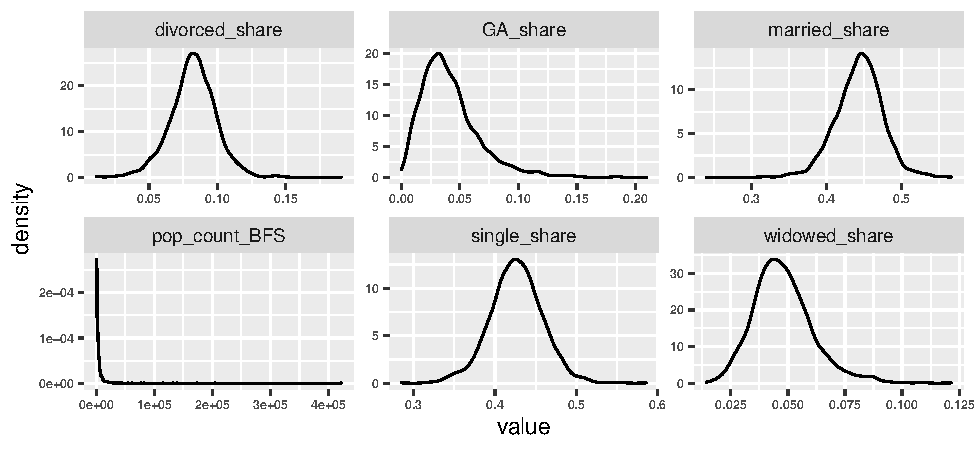
\includegraphics{Lin_Mod_Clus_Anal_files/figure-latex/unnamed-chunk-4-1.pdf}

\begin{Shaded}
\begin{Highlighting}[]
\NormalTok{d.inf\_fac[,}\DecValTok{11}\SpecialCharTok{:}\DecValTok{22}\NormalTok{] }\SpecialCharTok{\%\textgreater{}\%}
  \FunctionTok{keep}\NormalTok{(is.numeric) }\SpecialCharTok{\%\textgreater{}\%}
  \FunctionTok{gather}\NormalTok{() }\SpecialCharTok{\%\textgreater{}\%}
  \FunctionTok{ggplot}\NormalTok{(}\FunctionTok{aes}\NormalTok{(value))  }\SpecialCharTok{+}                   \CommentTok{\# Plot the values}
    \FunctionTok{facet\_wrap}\NormalTok{(}\SpecialCharTok{\textasciitilde{}}\NormalTok{ key, }\AttributeTok{scales =} \StringTok{"free"}\NormalTok{) }\SpecialCharTok{+}  \CommentTok{\# In separate panels}
    \FunctionTok{geom\_density}\NormalTok{() }\SpecialCharTok{+}                      \CommentTok{\# show density lines}
    \FunctionTok{theme}\NormalTok{(}\AttributeTok{axis.text=}\FunctionTok{element\_text}\NormalTok{(}\AttributeTok{size=}\DecValTok{6}\NormalTok{, }\AttributeTok{face=}\StringTok{"bold"}\NormalTok{)) }\CommentTok{\# change axis size}
\end{Highlighting}
\end{Shaded}

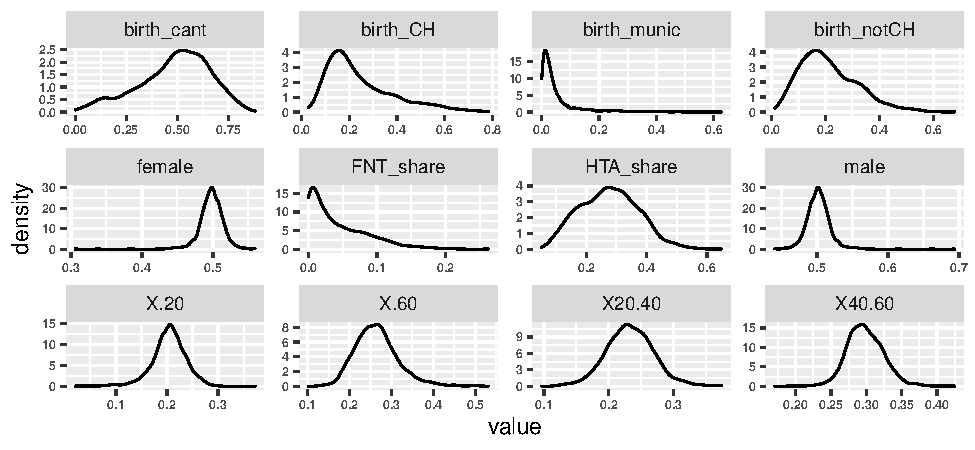
\includegraphics{Lin_Mod_Clus_Anal_files/figure-latex/unnamed-chunk-4-2.pdf}

\begin{Shaded}
\begin{Highlighting}[]
\NormalTok{d.inf\_fac[,}\DecValTok{23}\SpecialCharTok{:}\DecValTok{34}\NormalTok{] }\SpecialCharTok{\%\textgreater{}\%}
  \FunctionTok{keep}\NormalTok{(is.numeric) }\SpecialCharTok{\%\textgreater{}\%}
  \FunctionTok{gather}\NormalTok{() }\SpecialCharTok{\%\textgreater{}\%}
  \FunctionTok{ggplot}\NormalTok{(}\FunctionTok{aes}\NormalTok{(value))  }\SpecialCharTok{+}                   \CommentTok{\# Plot the values}
    \FunctionTok{facet\_wrap}\NormalTok{(}\SpecialCharTok{\textasciitilde{}}\NormalTok{ key, }\AttributeTok{scales =} \StringTok{"free"}\NormalTok{) }\SpecialCharTok{+}  \CommentTok{\# In separate panels}
    \FunctionTok{geom\_density}\NormalTok{() }\SpecialCharTok{+}                      \CommentTok{\# show density lines}
    \FunctionTok{theme}\NormalTok{(}\AttributeTok{axis.text=}\FunctionTok{element\_text}\NormalTok{(}\AttributeTok{size=}\DecValTok{6}\NormalTok{, }\AttributeTok{face=}\StringTok{"bold"}\NormalTok{)) }\CommentTok{\# change axis size}
\end{Highlighting}
\end{Shaded}

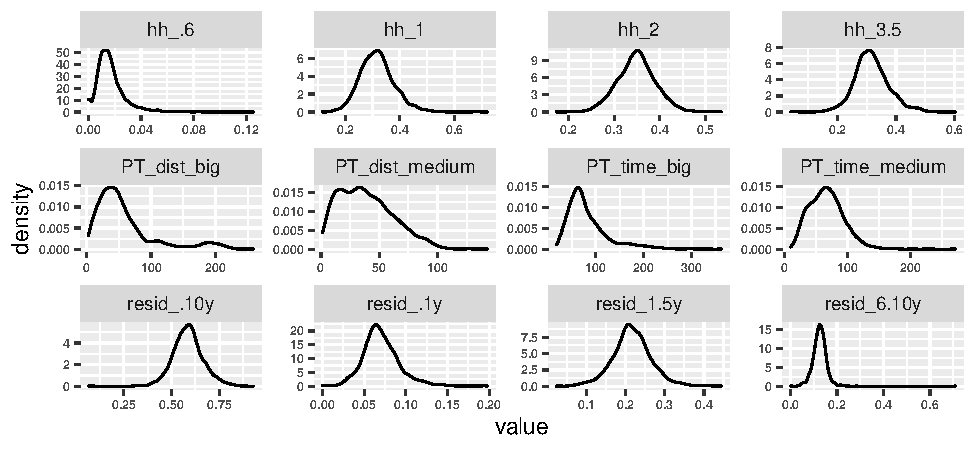
\includegraphics{Lin_Mod_Clus_Anal_files/figure-latex/unnamed-chunk-4-3.pdf}

\begin{Shaded}
\begin{Highlighting}[]
\NormalTok{d.inf\_fac[,}\DecValTok{35}\SpecialCharTok{:}\DecValTok{45}\NormalTok{] }\SpecialCharTok{\%\textgreater{}\%}
  \FunctionTok{keep}\NormalTok{(is.numeric) }\SpecialCharTok{\%\textgreater{}\%}
  \FunctionTok{gather}\NormalTok{() }\SpecialCharTok{\%\textgreater{}\%}
  \FunctionTok{ggplot}\NormalTok{(}\FunctionTok{aes}\NormalTok{(value))  }\SpecialCharTok{+}                   \CommentTok{\# Plot the values}
    \FunctionTok{facet\_wrap}\NormalTok{(}\SpecialCharTok{\textasciitilde{}}\NormalTok{ key, }\AttributeTok{scales =} \StringTok{"free"}\NormalTok{) }\SpecialCharTok{+}  \CommentTok{\# In separate panels}
    \FunctionTok{geom\_density}\NormalTok{() }\SpecialCharTok{+}                      \CommentTok{\# show density lines}
    \FunctionTok{theme}\NormalTok{(}\AttributeTok{axis.text=}\FunctionTok{element\_text}\NormalTok{(}\AttributeTok{size=}\DecValTok{6}\NormalTok{, }\AttributeTok{face=}\StringTok{"bold"}\NormalTok{)) }\CommentTok{\# change axis size}
\end{Highlighting}
\end{Shaded}

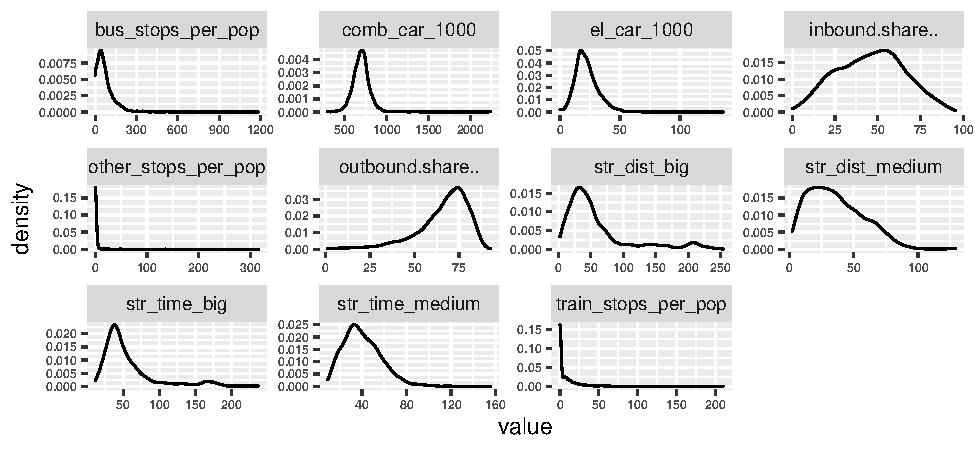
\includegraphics{Lin_Mod_Clus_Anal_files/figure-latex/unnamed-chunk-4-4.pdf}

\hypertarget{correlation-charts-to-factor-groups}{%
\subsection{Correlation charts to factor
groups}\label{correlation-charts-to-factor-groups}}

\hypertarget{marital-state}{%
\subsubsection{Marital state}\label{marital-state}}

\begin{Shaded}
\begin{Highlighting}[]
\FunctionTok{chart.Correlation}\NormalTok{(}\FunctionTok{log}\NormalTok{(d.inf\_fac[,}\FunctionTok{c}\NormalTok{(}\DecValTok{10}\SpecialCharTok{:}\DecValTok{12}\NormalTok{, }\DecValTok{6}\SpecialCharTok{:}\DecValTok{9}\NormalTok{)]}\SpecialCharTok{+}\DecValTok{1}\NormalTok{), }\CommentTok{\# +1 due to 0{-}values (log(0) = {-}Inf)}
                  \AttributeTok{histogram=}\ConstantTok{TRUE}\NormalTok{) }\CommentTok{\# adding histograms to the plot}
\end{Highlighting}
\end{Shaded}

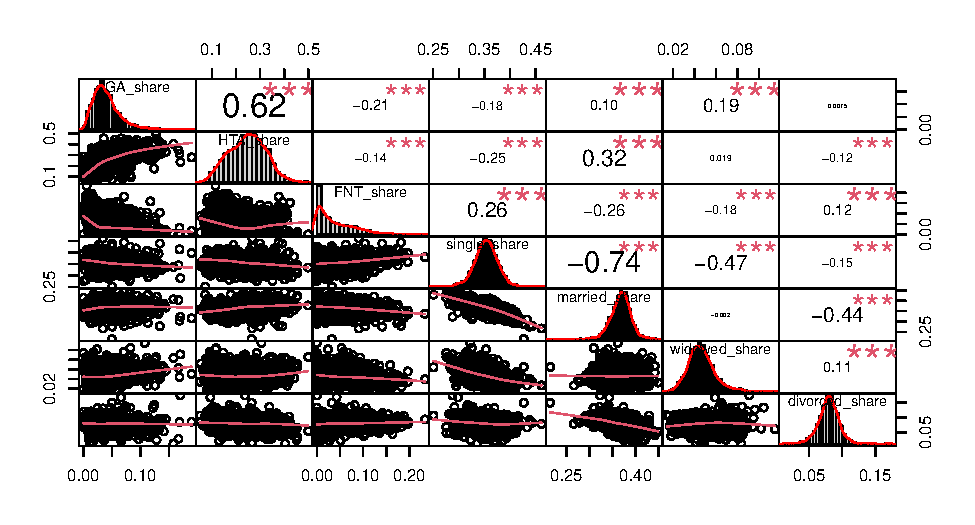
\includegraphics{Lin_Mod_Clus_Anal_files/figure-latex/unnamed-chunk-5-1.pdf}

\hypertarget{age-segment}{%
\subsubsection{Age segment}\label{age-segment}}

\begin{Shaded}
\begin{Highlighting}[]
\FunctionTok{chart.Correlation}\NormalTok{(}\FunctionTok{log}\NormalTok{(d.inf\_fac[,}\FunctionTok{c}\NormalTok{(}\DecValTok{10}\SpecialCharTok{:}\DecValTok{12}\NormalTok{, }\DecValTok{13}\SpecialCharTok{:}\DecValTok{16}\NormalTok{)]}\SpecialCharTok{+}\DecValTok{1}\NormalTok{), }\CommentTok{\# +1 due to 0{-}values (log(0) = {-}Inf)}
                  \AttributeTok{histogram=}\ConstantTok{TRUE}\NormalTok{) }\CommentTok{\# adding histograms to the plot}
\end{Highlighting}
\end{Shaded}

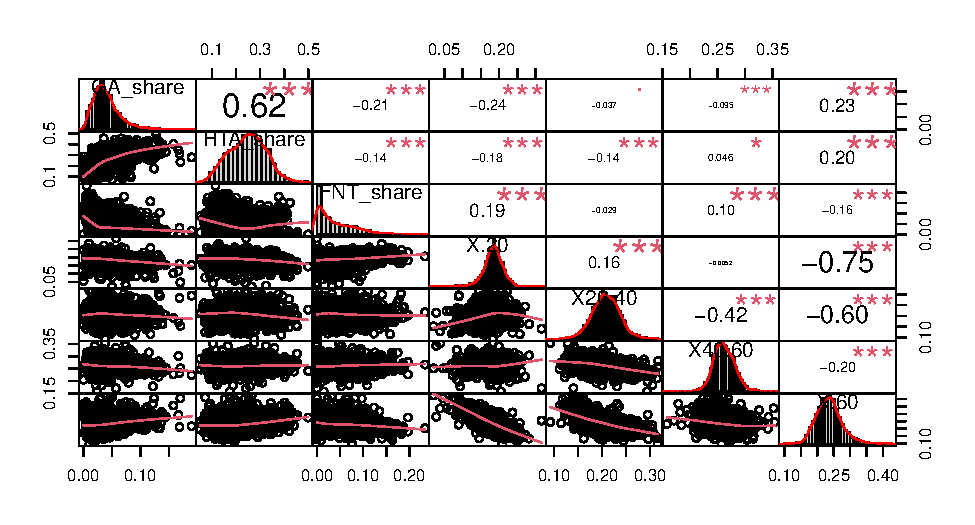
\includegraphics{Lin_Mod_Clus_Anal_files/figure-latex/unnamed-chunk-6-1.pdf}

\hypertarget{birth-origin}{%
\subsubsection{Birth origin}\label{birth-origin}}

\begin{Shaded}
\begin{Highlighting}[]
\FunctionTok{chart.Correlation}\NormalTok{(}\FunctionTok{log}\NormalTok{(d.inf\_fac[,}\FunctionTok{c}\NormalTok{(}\DecValTok{10}\SpecialCharTok{:}\DecValTok{12}\NormalTok{, }\DecValTok{17}\SpecialCharTok{:}\DecValTok{20}\NormalTok{)]}\SpecialCharTok{+}\DecValTok{1}\NormalTok{), }\CommentTok{\# +1 due to 0{-}values (log(0) = {-}Inf)}
                  \AttributeTok{histogram=}\ConstantTok{TRUE}\NormalTok{) }\CommentTok{\# adding histograms to the plot}
\end{Highlighting}
\end{Shaded}

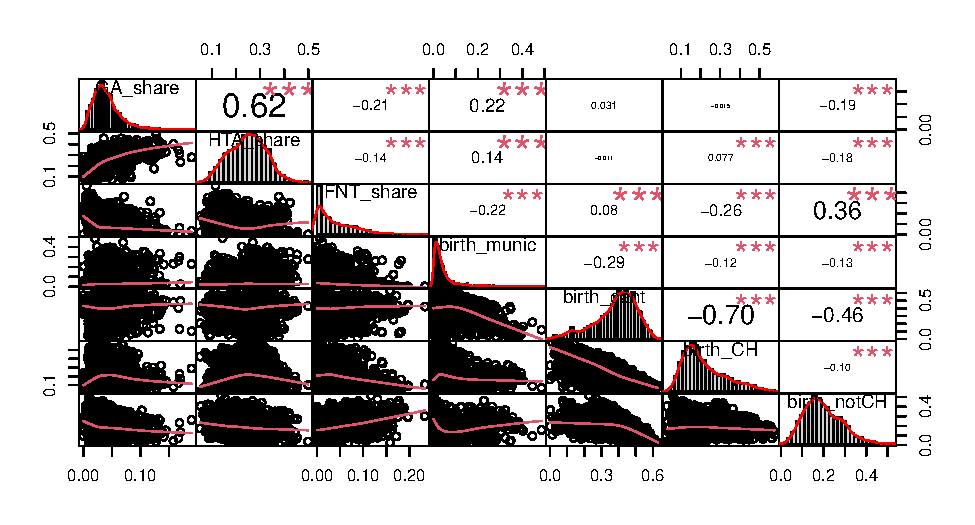
\includegraphics{Lin_Mod_Clus_Anal_files/figure-latex/unnamed-chunk-7-1.pdf}

\hypertarget{gender}{%
\subsubsection{Gender}\label{gender}}

\begin{Shaded}
\begin{Highlighting}[]
\FunctionTok{chart.Correlation}\NormalTok{(}\FunctionTok{log}\NormalTok{(d.inf\_fac[,}\FunctionTok{c}\NormalTok{(}\DecValTok{10}\SpecialCharTok{:}\DecValTok{12}\NormalTok{, }\DecValTok{21}\SpecialCharTok{:}\DecValTok{22}\NormalTok{)]}\SpecialCharTok{+}\DecValTok{1}\NormalTok{), }\CommentTok{\# +1 due to 0{-}values (log(0) = {-}Inf)}
                  \AttributeTok{histogram=}\ConstantTok{TRUE}\NormalTok{) }\CommentTok{\# adding histograms to the plot}
\end{Highlighting}
\end{Shaded}

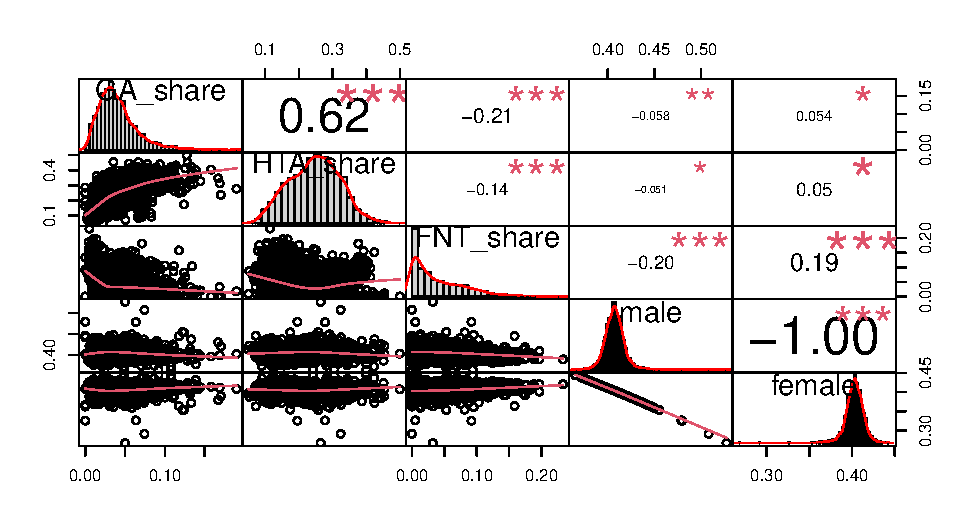
\includegraphics{Lin_Mod_Clus_Anal_files/figure-latex/unnamed-chunk-8-1.pdf}

\hypertarget{residence-time}{%
\subsubsection{Residence time}\label{residence-time}}

\begin{Shaded}
\begin{Highlighting}[]
\FunctionTok{chart.Correlation}\NormalTok{(}\FunctionTok{log}\NormalTok{(d.inf\_fac[,}\FunctionTok{c}\NormalTok{(}\DecValTok{10}\SpecialCharTok{:}\DecValTok{12}\NormalTok{, }\DecValTok{23}\SpecialCharTok{:}\DecValTok{26}\NormalTok{)]}\SpecialCharTok{+}\DecValTok{1}\NormalTok{), }\CommentTok{\# +1 due to 0{-}values (log(0) = {-}Inf)}
                  \AttributeTok{histogram=}\ConstantTok{TRUE}\NormalTok{) }\CommentTok{\# adding histograms to the plot}
\end{Highlighting}
\end{Shaded}

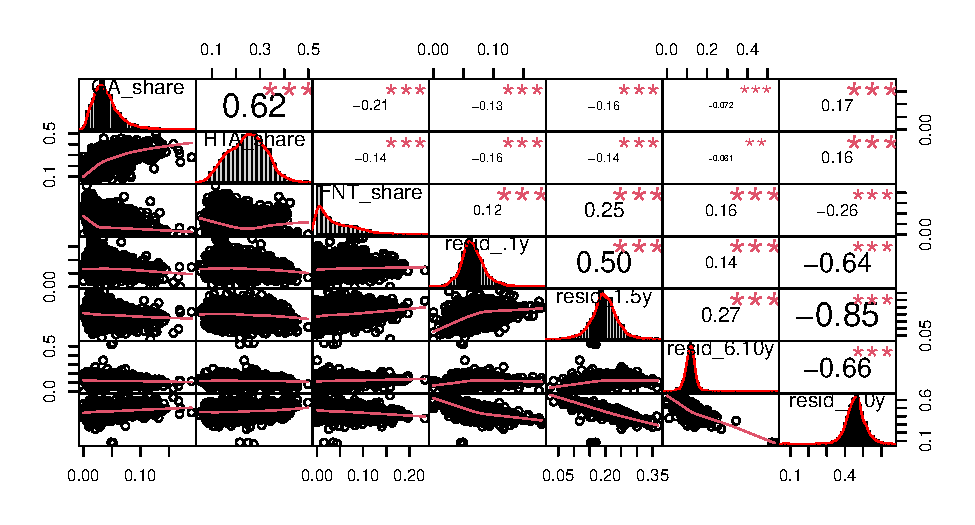
\includegraphics{Lin_Mod_Clus_Anal_files/figure-latex/unnamed-chunk-9-1.pdf}

\hypertarget{household-size}{%
\subsubsection{Household size}\label{household-size}}

\begin{Shaded}
\begin{Highlighting}[]
\FunctionTok{chart.Correlation}\NormalTok{(}\FunctionTok{log}\NormalTok{(d.inf\_fac[,}\FunctionTok{c}\NormalTok{(}\DecValTok{10}\SpecialCharTok{:}\DecValTok{12}\NormalTok{, }\DecValTok{27}\SpecialCharTok{:}\DecValTok{30}\NormalTok{)]}\SpecialCharTok{+}\DecValTok{1}\NormalTok{), }\CommentTok{\# +1 due to 0{-}values (log(0) = {-}Inf)}
                  \AttributeTok{histogram=}\ConstantTok{TRUE}\NormalTok{) }\CommentTok{\# adding histograms to the plot}
\end{Highlighting}
\end{Shaded}

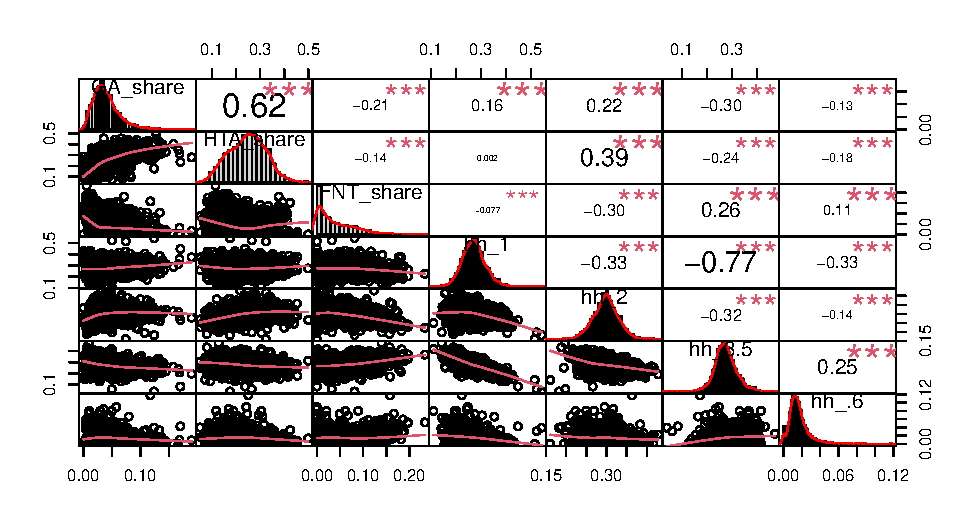
\includegraphics{Lin_Mod_Clus_Anal_files/figure-latex/unnamed-chunk-10-1.pdf}

\hypertarget{pt-distance-and-time-to-middlebig-cities}{%
\subsubsection{PT Distance and time to middle/big
cities}\label{pt-distance-and-time-to-middlebig-cities}}

\begin{Shaded}
\begin{Highlighting}[]
\FunctionTok{chart.Correlation}\NormalTok{(}\FunctionTok{log}\NormalTok{(d.inf\_fac[,}\FunctionTok{c}\NormalTok{(}\DecValTok{10}\SpecialCharTok{:}\DecValTok{12}\NormalTok{, }\DecValTok{31}\SpecialCharTok{:}\DecValTok{34}\NormalTok{)]}\SpecialCharTok{+}\DecValTok{1}\NormalTok{), }\CommentTok{\# +1 due to 0{-}values (log(0) = {-}Inf)}
                  \AttributeTok{histogram=}\ConstantTok{TRUE}\NormalTok{) }\CommentTok{\# adding histograms to the plot}
\end{Highlighting}
\end{Shaded}

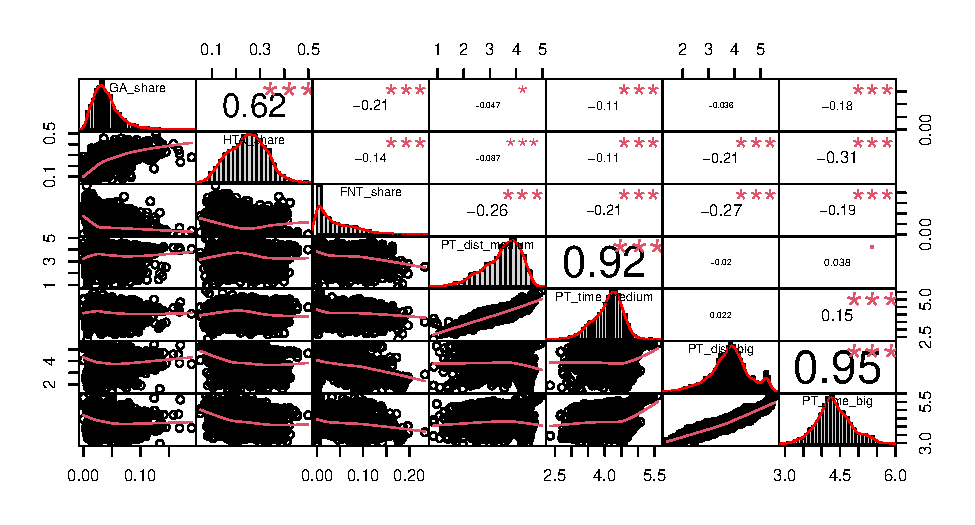
\includegraphics{Lin_Mod_Clus_Anal_files/figure-latex/unnamed-chunk-11-1.pdf}

\hypertarget{bus-train-other-stops-per-population}{%
\subsubsection{Bus / train / other stops per
population}\label{bus-train-other-stops-per-population}}

\begin{Shaded}
\begin{Highlighting}[]
\FunctionTok{chart.Correlation}\NormalTok{(}\FunctionTok{log}\NormalTok{(d.inf\_fac[,}\FunctionTok{c}\NormalTok{(}\DecValTok{10}\SpecialCharTok{:}\DecValTok{12}\NormalTok{, }\DecValTok{5}\NormalTok{, }\DecValTok{39}\SpecialCharTok{:}\DecValTok{41}\NormalTok{)]}\SpecialCharTok{+}\DecValTok{1}\NormalTok{), }\CommentTok{\# +1 due to 0{-}values (log(0) = {-}Inf)}
                  \AttributeTok{histogram=}\ConstantTok{TRUE}\NormalTok{) }\CommentTok{\# adding histograms to the plot}
\end{Highlighting}
\end{Shaded}

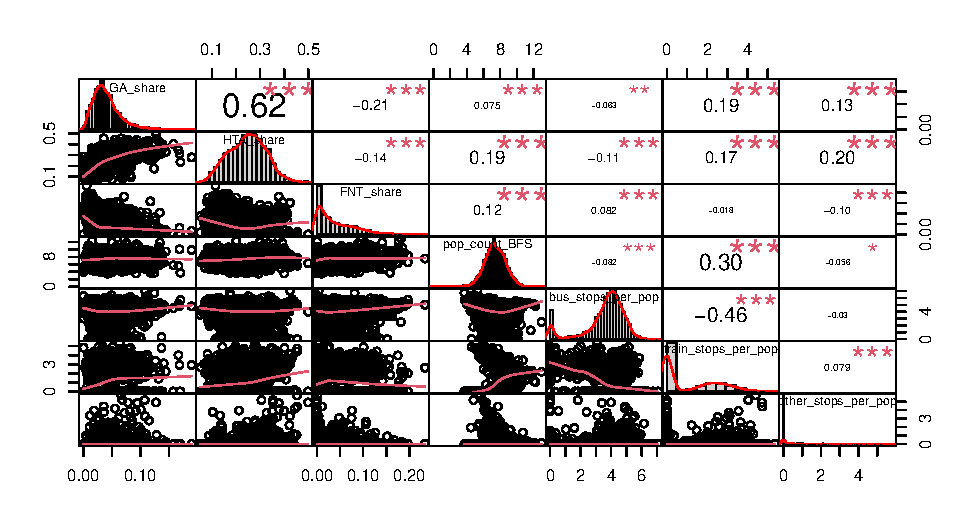
\includegraphics{Lin_Mod_Clus_Anal_files/figure-latex/unnamed-chunk-12-1.pdf}

\hypertarget{car-distribution}{%
\subsubsection{Car distribution}\label{car-distribution}}

\begin{Shaded}
\begin{Highlighting}[]
\FunctionTok{chart.Correlation}\NormalTok{(}\FunctionTok{log}\NormalTok{(d.inf\_fac[,}\FunctionTok{c}\NormalTok{(}\DecValTok{10}\SpecialCharTok{:}\DecValTok{12}\NormalTok{, }\DecValTok{42}\SpecialCharTok{:}\DecValTok{43}\NormalTok{)]}\SpecialCharTok{+}\DecValTok{1}\NormalTok{), }\CommentTok{\# +1 due to 0{-}values (log(0) = {-}Inf)}
                  \AttributeTok{histogram=}\ConstantTok{TRUE}\NormalTok{) }\CommentTok{\# adding histograms to the plot}
\end{Highlighting}
\end{Shaded}

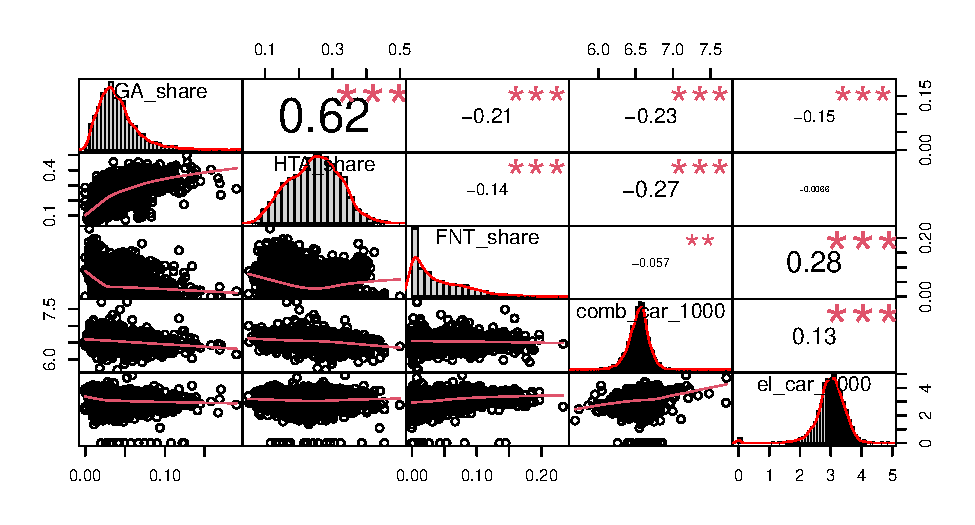
\includegraphics{Lin_Mod_Clus_Anal_files/figure-latex/unnamed-chunk-13-1.pdf}

\hypertarget{commuter-statistics}{%
\subsubsection{Commuter statistics}\label{commuter-statistics}}

\begin{Shaded}
\begin{Highlighting}[]
\FunctionTok{chart.Correlation}\NormalTok{(}\FunctionTok{log}\NormalTok{(d.inf\_fac[,}\FunctionTok{c}\NormalTok{(}\DecValTok{10}\SpecialCharTok{:}\DecValTok{12}\NormalTok{, }\DecValTok{44}\SpecialCharTok{:}\DecValTok{45}\NormalTok{)]}\SpecialCharTok{+}\DecValTok{1}\NormalTok{), }\CommentTok{\# +1 due to 0{-}values (log(0) = {-}Inf)}
                  \AttributeTok{histogram=}\ConstantTok{TRUE}\NormalTok{) }\CommentTok{\# adding histograms to the plot}
\end{Highlighting}
\end{Shaded}

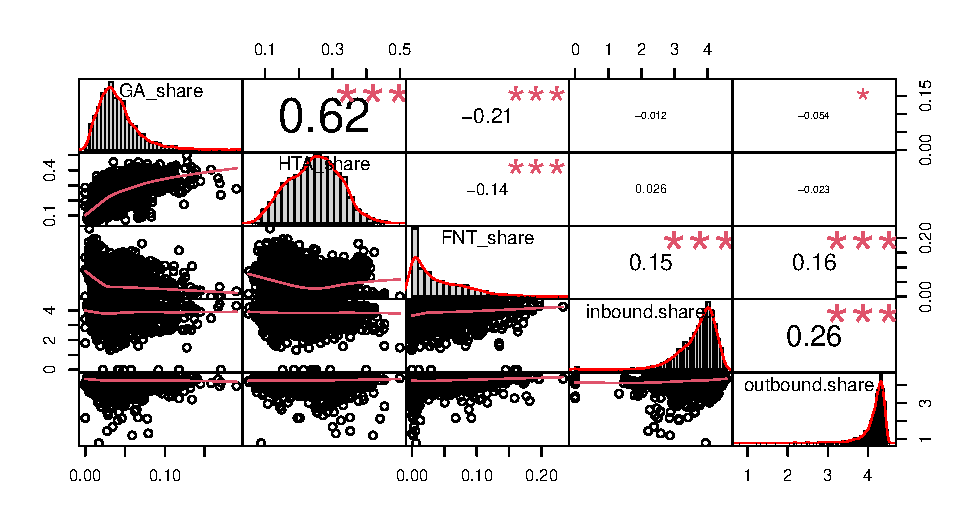
\includegraphics{Lin_Mod_Clus_Anal_files/figure-latex/unnamed-chunk-14-1.pdf}

\hypertarget{ga-hta-fnt-shares-compared-to-languages}{%
\subsection{GA, HTA \& FNT shares compared to
languages:}\label{ga-hta-fnt-shares-compared-to-languages}}

\begin{Shaded}
\begin{Highlighting}[]
\NormalTok{plot\_HTA }\OtherTok{\textless{}{-}} \FunctionTok{ggbarplot}\NormalTok{(d.inf\_fac, }\AttributeTok{x=}\StringTok{"language"}\NormalTok{, }\AttributeTok{y=}\StringTok{"HTA\_share"}\NormalTok{, }
                      \AttributeTok{fill=}\StringTok{"language"}\NormalTok{, }
              \CommentTok{\#        facet.by="language", }
                      \AttributeTok{add =} \StringTok{"mean\_se"}\NormalTok{,}
                      \AttributeTok{xlab =} \StringTok{"language"}\NormalTok{,}
                      \AttributeTok{legend =} \StringTok{"right"}\NormalTok{,}
                      \AttributeTok{title =} \StringTok{"HTA"}\NormalTok{,}
                      \AttributeTok{ggtheme =} \FunctionTok{theme\_cleveland}\NormalTok{()) }\SpecialCharTok{+} \CommentTok{\# better looking theme}
  \FunctionTok{theme}\NormalTok{(}\AttributeTok{axis.text=}\FunctionTok{element\_text}\NormalTok{(}\AttributeTok{size=}\FloatTok{6.5}\NormalTok{, }\AttributeTok{face=}\StringTok{"bold"}\NormalTok{))}

\NormalTok{plot\_GA }\OtherTok{\textless{}{-}} \FunctionTok{ggbarplot}\NormalTok{(d.inf\_fac, }\AttributeTok{x=}\StringTok{"language"}\NormalTok{, }\AttributeTok{y=}\StringTok{"GA\_share"}\NormalTok{, }
                      \AttributeTok{fill=}\StringTok{"language"}\NormalTok{, }
                \CommentTok{\#       facet.by="language", }
                      \AttributeTok{add =} \StringTok{"mean\_se"}\NormalTok{,}
                      \AttributeTok{xlab =} \StringTok{"language"}\NormalTok{,}
                      \AttributeTok{legend =} \StringTok{"right"}\NormalTok{,}
                      \AttributeTok{title =} \StringTok{"GA"}\NormalTok{,}
                      \AttributeTok{ggtheme =} \FunctionTok{theme\_cleveland}\NormalTok{()) }\SpecialCharTok{+}
  \FunctionTok{theme}\NormalTok{(}\AttributeTok{axis.text=}\FunctionTok{element\_text}\NormalTok{(}\AttributeTok{size=}\FloatTok{6.5}\NormalTok{, }\AttributeTok{face=}\StringTok{"bold"}\NormalTok{))}

\NormalTok{plot\_FNT }\OtherTok{\textless{}{-}} \FunctionTok{ggbarplot}\NormalTok{(d.inf\_fac, }\AttributeTok{x=}\StringTok{"language"}\NormalTok{, }\AttributeTok{y=}\StringTok{"FNT\_share"}\NormalTok{, }
                      \AttributeTok{fill=}\StringTok{"language"}\NormalTok{, }
                    \CommentTok{\#  facet.by="language", }
                      \AttributeTok{add =} \StringTok{"mean\_se"}\NormalTok{,}
                      \AttributeTok{xlab =} \StringTok{"language"}\NormalTok{,}
                      \AttributeTok{legend =} \StringTok{"right"}\NormalTok{,}
                      \AttributeTok{title =} \StringTok{"FNT"}\NormalTok{,}
                      \AttributeTok{ggtheme =} \FunctionTok{theme\_cleveland}\NormalTok{()) }\SpecialCharTok{+}
  \FunctionTok{theme}\NormalTok{(}\AttributeTok{axis.text=}\FunctionTok{element\_text}\NormalTok{(}\AttributeTok{size=}\FloatTok{6.5}\NormalTok{, }\AttributeTok{face=}\StringTok{"bold"}\NormalTok{))}


\NormalTok{share.comparison }\OtherTok{\textless{}{-}} \FunctionTok{ggarrange}\NormalTok{(plot\_GA, plot\_HTA, plot\_FNT, }\AttributeTok{ncol=}\DecValTok{3}\NormalTok{) }\CommentTok{\# two plots beside each other}

\FunctionTok{annotate\_figure}\NormalTok{(share.comparison, }
                \AttributeTok{top =} \FunctionTok{text\_grob}\NormalTok{(}\StringTok{"Comparison of mean share of GA \& }
\StringTok{                                HTA sold in \% of population"}\NormalTok{, }
                                \AttributeTok{face =} \StringTok{"bold"}\NormalTok{)) }\CommentTok{\# set over{-}all title ("top")}
\end{Highlighting}
\end{Shaded}

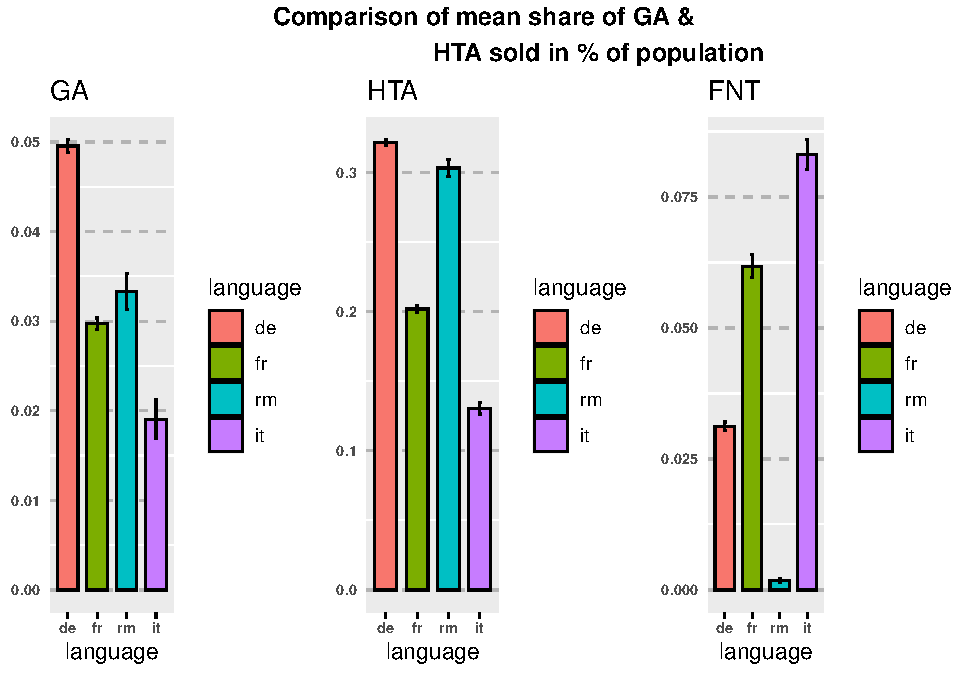
\includegraphics{Lin_Mod_Clus_Anal_files/figure-latex/unnamed-chunk-15-1.pdf}

\newpage

\hypertarget{modelling-shares}{%
\section{MODELLING SHARES}\label{modelling-shares}}

I will achieve the first objective of modelling the share of season
tickets through two different approaches:

\hypertarget{train-test-splitting}{%
\subsection{Train / Test splitting}\label{train-test-splitting}}

\begin{Shaded}
\begin{Highlighting}[]
\FunctionTok{set.seed}\NormalTok{(}\DecValTok{234}\NormalTok{) }\CommentTok{\# reproducible}
\NormalTok{indexes }\OtherTok{\textless{}{-}} \FunctionTok{createDataPartition}\NormalTok{(d.inf\_fac}\SpecialCharTok{$}\NormalTok{BFS\_Nr, }\AttributeTok{p =}\NormalTok{ .}\DecValTok{8}\NormalTok{, }\AttributeTok{list =} \ConstantTok{FALSE}\NormalTok{) }
\NormalTok{d.train }\OtherTok{\textless{}{-}}\NormalTok{ d.inf\_fac[indexes, ]}
\NormalTok{d.test }\OtherTok{\textless{}{-}}\NormalTok{ d.inf\_fac[}\SpecialCharTok{{-}}\NormalTok{indexes, ]}

\FunctionTok{sum}\NormalTok{(}\FunctionTok{length}\NormalTok{(d.train}\SpecialCharTok{$}\NormalTok{BFS\_Nr) }\SpecialCharTok{+} \FunctionTok{length}\NormalTok{(d.test}\SpecialCharTok{$}\NormalTok{BFS\_Nr)) }\CommentTok{\# control the split}
\end{Highlighting}
\end{Shaded}

\begin{verbatim}
## [1] 2148
\end{verbatim}

\begin{Shaded}
\begin{Highlighting}[]
\FunctionTok{length}\NormalTok{(d.inf\_fac}\SpecialCharTok{$}\NormalTok{BFS\_Nr)}
\end{Highlighting}
\end{Shaded}

\begin{verbatim}
## [1] 2148
\end{verbatim}

\begin{Shaded}
\begin{Highlighting}[]
\CommentTok{\# print(d.train[1:5,])}
\end{Highlighting}
\end{Shaded}

\hypertarget{function-for-model-evaluation}{%
\subsection{Function for Model
Evaluation}\label{function-for-model-evaluation}}

For the evaluation of our models we will use the following function,
which displays the RMSE and the R\_squared for our predicted values.
Furthermore, we will use cross validation in order to find the best
fitting model.

\begin{Shaded}
\begin{Highlighting}[]
\NormalTok{eval\_results }\OtherTok{\textless{}{-}} \ControlFlowTok{function}\NormalTok{(true, predicted) \{}
\NormalTok{  SSE }\OtherTok{\textless{}{-}} \FunctionTok{sum}\NormalTok{((predicted }\SpecialCharTok{{-}}\NormalTok{ true)}\SpecialCharTok{\^{}}\DecValTok{2}\NormalTok{, }\AttributeTok{na.rm =} \ConstantTok{TRUE}\NormalTok{)}
\NormalTok{  SST }\OtherTok{\textless{}{-}} \FunctionTok{sum}\NormalTok{((true }\SpecialCharTok{{-}} \FunctionTok{mean}\NormalTok{(true, }\AttributeTok{na.rm =} \ConstantTok{TRUE}\NormalTok{))}\SpecialCharTok{\^{}}\DecValTok{2}\NormalTok{, }\AttributeTok{na.rm =} \ConstantTok{TRUE}\NormalTok{)}
\NormalTok{  R\_square }\OtherTok{\textless{}{-}} \DecValTok{1} \SpecialCharTok{{-}}\NormalTok{ SSE }\SpecialCharTok{/}\NormalTok{ SST}
\NormalTok{  RMSE }\OtherTok{=} \FunctionTok{sqrt}\NormalTok{(SSE}\SpecialCharTok{/}\FunctionTok{length}\NormalTok{(true))}

\CommentTok{\# Model performance metrics}
\FunctionTok{data.frame}\NormalTok{(}\AttributeTok{RMSE =}\NormalTok{ RMSE,}
           \AttributeTok{Rsquare =}\NormalTok{ R\_square)}
\NormalTok{\}}
\end{Highlighting}
\end{Shaded}

\hypertarget{linear-model}{%
\subsection{Linear model}\label{linear-model}}

The first method is a classic linear model that models the absolute
number of season tickets in circulation. A special eye must be kept on
the possible interactions between the variables, wherefore I will
include the interactions in the model at the beginning. By using the
Akaike Information Criteria (AIC), I can assess afterwards which
variables explain the model most meaningfully. Additionally, normalizing
data must be taken into account.

\hypertarget{building-linear-model-with-all-variables}{%
\subsubsection{Building linear model with all
variables}\label{building-linear-model-with-all-variables}}

\begin{Shaded}
\begin{Highlighting}[]
\NormalTok{lm0 }\OtherTok{\textless{}{-}} \FunctionTok{lm}\NormalTok{(GA\_share }\SpecialCharTok{\textasciitilde{}}\NormalTok{ . }\SpecialCharTok{{-}}\NormalTok{HTA\_share }\SpecialCharTok{{-}}\NormalTok{ FNT\_share, }\AttributeTok{data =}\NormalTok{ d.train[, }\DecValTok{4}\SpecialCharTok{:}\DecValTok{45}\NormalTok{]) }\CommentTok{\# Model with all predictors}
\FunctionTok{summary}\NormalTok{(lm0)}
\end{Highlighting}
\end{Shaded}

\begin{verbatim}
## 
## Call:
## lm(formula = GA_share ~ . - HTA_share - FNT_share, data = d.train[, 
##     4:45])
## 
## Residuals:
##       Min        1Q    Median        3Q       Max 
## -0.063432 -0.012548 -0.002048  0.009790  0.136964 
## 
## Coefficients: (4 not defined because of singularities)
##                       Estimate Std. Error t value Pr(>|t|)    
## (Intercept)          2.941e+00  4.632e+00   0.635  0.52556    
## languagefr          -1.418e-02  1.868e-03  -7.590 5.53e-14 ***
## languageit          -5.381e-02  4.771e-03 -11.279  < 2e-16 ***
## languagerm          -1.858e-02  4.313e-03  -4.307 1.76e-05 ***
## pop_count_BFS        4.778e-08  4.234e-08   1.128  0.25934    
## single_share        -3.101e+00  4.626e+00  -0.670  0.50276    
## married_share       -3.164e+00  4.625e+00  -0.684  0.49407    
## widowed_share       -3.189e+00  4.624e+00  -0.690  0.49045    
## divorced_share      -3.093e+00  4.626e+00  -0.669  0.50389    
## X.20                -1.594e-01  3.425e-02  -4.654 3.54e-06 ***
## X20.40              -1.163e-01  2.610e-02  -4.455 9.00e-06 ***
## X40.60              -8.685e-02  2.941e-02  -2.953  0.00319 ** 
## X.60                        NA         NA      NA       NA    
## birth_munic          1.020e-01  1.197e-02   8.521  < 2e-16 ***
## birth_cant           6.428e-02  8.325e-03   7.722 2.06e-14 ***
## birth_CH             5.456e-02  9.132e-03   5.975 2.86e-09 ***
## birth_notCH                 NA         NA      NA       NA    
## male                -4.489e-02  3.380e-02  -1.328  0.18438    
## female                      NA         NA      NA       NA    
## resid_.1y            2.708e-01  2.026e-01   1.337  0.18154    
## resid_1.5y           2.575e-01  2.019e-01   1.275  0.20249    
## resid_6.10y          3.113e-01  2.025e-01   1.538  0.12437    
## resid_.10y           2.338e-01  2.016e-01   1.159  0.24644    
## hh_1                 1.003e-01  5.751e-02   1.745  0.08122 .  
## hh_2                 3.186e-02  5.982e-02   0.533  0.59436    
## hh_3.5               6.365e-02  5.957e-02   1.069  0.28543    
## hh_.6                       NA         NA      NA       NA    
## PT_dist_medium       1.381e-05  1.048e-04   0.132  0.89524    
## PT_time_medium      -1.256e-04  6.906e-05  -1.818  0.06920 .  
## PT_dist_big         -1.519e-04  9.678e-05  -1.570  0.11665    
## PT_time_big         -3.512e-04  6.508e-05  -5.397 7.85e-08 ***
## str_dist_medium     -4.259e-05  1.133e-04  -0.376  0.70712    
## str_time_medium      5.848e-05  1.160e-04   0.504  0.61427    
## str_dist_big         1.978e-04  8.540e-05   2.316  0.02066 *  
## str_time_big         3.968e-04  1.012e-04   3.922 9.17e-05 ***
## bus_stops_per_pop    3.301e-05  8.441e-06   3.910 9.63e-05 ***
## train_stops_per_pop  1.656e-04  3.519e-05   4.705 2.76e-06 ***
## other_stops_per_pop -5.565e-06  4.661e-05  -0.119  0.90497    
## comb_car_1000       -2.880e-05  5.638e-06  -5.109 3.65e-07 ***
## el_car_1000          1.212e-04  6.290e-05   1.926  0.05429 .  
## inbound.share..      3.175e-05  3.552e-05   0.894  0.37147    
## outbound.share..     1.083e-04  5.509e-05   1.966  0.04944 *  
## ---
## Signif. codes:  0 '***' 0.001 '**' 0.01 '*' 0.05 '.' 0.1 ' ' 1
## 
## Residual standard error: 0.01965 on 1532 degrees of freedom
##   (150 observations deleted due to missingness)
## Multiple R-squared:  0.4243, Adjusted R-squared:  0.4104 
## F-statistic: 30.52 on 37 and 1532 DF,  p-value: < 2.2e-16
\end{verbatim}

\begin{Shaded}
\begin{Highlighting}[]
\NormalTok{MASS}\SpecialCharTok{::}\FunctionTok{stepAIC}\NormalTok{(lm0, }\AttributeTok{direction =} \StringTok{"both"}\NormalTok{, }\AttributeTok{trace =} \ConstantTok{FALSE}\NormalTok{)}
\end{Highlighting}
\end{Shaded}

\begin{verbatim}
## 
## Call:
## lm(formula = GA_share ~ language + married_share + widowed_share + 
##     X.20 + X20.40 + X40.60 + birth_munic + birth_cant + birth_CH + 
##     male + resid_1.5y + resid_6.10y + hh_1 + PT_time_medium + 
##     PT_dist_big + PT_time_big + str_dist_big + str_time_big + 
##     bus_stops_per_pop + train_stops_per_pop + comb_car_1000 + 
##     el_car_1000 + outbound.share.., data = d.train[, 4:45])
## 
## Coefficients:
##         (Intercept)           languagefr           languageit  
##           1.230e-01           -1.364e-02           -5.262e-02  
##          languagerm        married_share        widowed_share  
##          -1.777e-02           -7.012e-02           -9.913e-02  
##                X.20               X20.40               X40.60  
##          -1.487e-01           -9.568e-02           -7.010e-02  
##         birth_munic           birth_cant             birth_CH  
##           9.837e-02            5.937e-02            4.981e-02  
##                male           resid_1.5y          resid_6.10y  
##          -5.101e-02            2.353e-02            7.702e-02  
##                hh_1       PT_time_medium          PT_dist_big  
##           5.475e-02           -1.131e-04           -1.418e-04  
##         PT_time_big         str_dist_big         str_time_big  
##          -3.615e-04            1.850e-04            4.125e-04  
##   bus_stops_per_pop  train_stops_per_pop        comb_car_1000  
##           3.280e-05            1.681e-04           -2.992e-05  
##         el_car_1000     outbound.share..  
##           1.405e-04            1.259e-04
\end{verbatim}

The stepAIC function gives me now a suggested formula, what can be used
for a second try. The coefficients show the weights.

\hypertarget{building-linear-model-with-selected-variables}{%
\subsubsection{Building linear model with selected
variables}\label{building-linear-model-with-selected-variables}}

\begin{Shaded}
\begin{Highlighting}[]
\CommentTok{\# According to the stepAIC function we get this linear model}
\NormalTok{lm1 }\OtherTok{\textless{}{-}} \FunctionTok{lm}\NormalTok{(GA\_share }\SpecialCharTok{\textasciitilde{}}\NormalTok{ language }\SpecialCharTok{+}\NormalTok{ married\_share }\SpecialCharTok{+}\NormalTok{ widowed\_share }\SpecialCharTok{+} 
\NormalTok{    X}\FloatTok{.20} \SpecialCharTok{+}\NormalTok{ X20}\FloatTok{.40} \SpecialCharTok{+}\NormalTok{ X40}\FloatTok{.60} \SpecialCharTok{+}\NormalTok{ birth\_munic }\SpecialCharTok{+}\NormalTok{ birth\_cant }\SpecialCharTok{+}\NormalTok{ birth\_CH }\SpecialCharTok{+} 
\NormalTok{    male }\SpecialCharTok{+}\NormalTok{ resid\_1}\FloatTok{.5}\NormalTok{y }\SpecialCharTok{+}\NormalTok{ resid\_6}\FloatTok{.10}\NormalTok{y }\SpecialCharTok{+}\NormalTok{ hh\_1 }\SpecialCharTok{+}\NormalTok{ PT\_time\_medium }\SpecialCharTok{+} 
\NormalTok{    PT\_dist\_big }\SpecialCharTok{+}\NormalTok{ PT\_time\_big }\SpecialCharTok{+}\NormalTok{ str\_dist\_big }\SpecialCharTok{+}\NormalTok{ str\_time\_big }\SpecialCharTok{+} 
\NormalTok{    bus\_stops\_per\_pop }\SpecialCharTok{+}\NormalTok{ train\_stops\_per\_pop }\SpecialCharTok{+}\NormalTok{ comb\_car\_1000 }\SpecialCharTok{+} 
\NormalTok{    el\_car\_1000 }\SpecialCharTok{+}\NormalTok{ outbound.share.., }\AttributeTok{data =}\NormalTok{ d.train[, }\DecValTok{4}\SpecialCharTok{:}\DecValTok{45}\NormalTok{]) }
\FunctionTok{summary}\NormalTok{(lm1)}
\end{Highlighting}
\end{Shaded}

\begin{verbatim}
## 
## Call:
## lm(formula = GA_share ~ language + married_share + widowed_share + 
##     X.20 + X20.40 + X40.60 + birth_munic + birth_cant + birth_CH + 
##     male + resid_1.5y + resid_6.10y + hh_1 + PT_time_medium + 
##     PT_dist_big + PT_time_big + str_dist_big + str_time_big + 
##     bus_stops_per_pop + train_stops_per_pop + comb_car_1000 + 
##     el_car_1000 + outbound.share.., data = d.train[, 4:45])
## 
## Residuals:
##       Min        1Q    Median        3Q       Max 
## -0.060967 -0.012861 -0.002056  0.009822  0.132757 
## 
## Coefficients:
##                       Estimate Std. Error t value Pr(>|t|)    
## (Intercept)          1.230e-01  3.264e-02   3.767 0.000172 ***
## languagefr          -1.364e-02  1.544e-03  -8.832  < 2e-16 ***
## languageit          -5.262e-02  4.577e-03 -11.499  < 2e-16 ***
## languagerm          -1.777e-02  4.267e-03  -4.165 3.28e-05 ***
## married_share       -7.012e-02  2.630e-02  -2.666 0.007754 ** 
## widowed_share       -9.913e-02  6.821e-02  -1.453 0.146295    
## X.20                -1.487e-01  2.638e-02  -5.638 2.04e-08 ***
## X20.40              -9.568e-02  2.227e-02  -4.296 1.85e-05 ***
## X40.60              -7.010e-02  2.680e-02  -2.616 0.008989 ** 
## birth_munic          9.837e-02  1.089e-02   9.033  < 2e-16 ***
## birth_cant           5.937e-02  6.906e-03   8.597  < 2e-16 ***
## birth_CH             4.981e-02  7.766e-03   6.413 1.89e-10 ***
## male                -5.101e-02  3.288e-02  -1.552 0.120956    
## resid_1.5y           2.353e-02  1.409e-02   1.670 0.095167 .  
## resid_6.10y          7.702e-02  2.056e-02   3.747 0.000186 ***
## hh_1                 5.475e-02  1.538e-02   3.560 0.000382 ***
## PT_time_medium      -1.131e-04  2.299e-05  -4.920 9.57e-07 ***
## PT_dist_big         -1.418e-04  8.957e-05  -1.583 0.113686    
## PT_time_big         -3.615e-04  5.538e-05  -6.528 9.05e-11 ***
## str_dist_big         1.850e-04  7.873e-05   2.350 0.018909 *  
## str_time_big         4.125e-04  8.477e-05   4.866 1.26e-06 ***
## bus_stops_per_pop    3.280e-05  8.160e-06   4.019 6.13e-05 ***
## train_stops_per_pop  1.681e-04  3.405e-05   4.936 8.85e-07 ***
## comb_car_1000       -2.992e-05  5.438e-06  -5.502 4.40e-08 ***
## el_car_1000          1.405e-04  6.179e-05   2.274 0.023114 *  
## outbound.share..     1.259e-04  5.224e-05   2.410 0.016064 *  
## ---
## Signif. codes:  0 '***' 0.001 '**' 0.01 '*' 0.05 '.' 0.1 ' ' 1
## 
## Residual standard error: 0.01962 on 1544 degrees of freedom
##   (150 observations deleted due to missingness)
## Multiple R-squared:  0.4214, Adjusted R-squared:  0.412 
## F-statistic: 44.97 on 25 and 1544 DF,  p-value: < 2.2e-16
\end{verbatim}

\hypertarget{generalized-linear-model-with-family-binomial}{%
\subsection{Generalized Linear model with family
``Binomial''}\label{generalized-linear-model-with-family-binomial}}

\hypertarget{glm-binomial-with-all-data}{%
\subsubsection{GLM binomial with all
data}\label{glm-binomial-with-all-data}}

With a linear model, no probability distributions can be predicted, as
values above 1 and below 0 are possible, resulting in meaningless values
concerning the share. Therefore, a second, logistic approach comes into
play, which strictly forecasts values between 0 and 1. Although I do not
have values for individuals with regard to the share and thus do not
model a binary target variable, a multinomial logit model approach is
described for aggregated data using group variable, which is in my case
the municipality (Morais et al., 2016). Quasibinomial glm fulfills the
criteria here:

See here:
\url{https://stats.oarc.ucla.edu/r/dae/multinomial-logistic-regression/\#}:\textasciitilde:text=Multinomial\%20logistic\%20regression\%20is\%20used,the\%20examples\%20on\%20this\%20page.

\begin{Shaded}
\begin{Highlighting}[]
\CommentTok{\# Setting up model with all data}

\NormalTok{glmodel0 }\OtherTok{\textless{}{-}} \FunctionTok{glm}\NormalTok{(GA\_share }\SpecialCharTok{\textasciitilde{}}\NormalTok{ . }\SpecialCharTok{{-}}\NormalTok{HTA\_share}
              \SpecialCharTok{{-}}\NormalTok{ FNT\_share, }\AttributeTok{family =}\NormalTok{ quasibinomial, }\AttributeTok{data=}\NormalTok{d.train[,}\DecValTok{4}\SpecialCharTok{:}\DecValTok{45}\NormalTok{])}
\FunctionTok{summary}\NormalTok{(glmodel0)}
\end{Highlighting}
\end{Shaded}

\begin{verbatim}
## 
## Call:
## glm(formula = GA_share ~ . - HTA_share - FNT_share, family = quasibinomial, 
##     data = d.train[, 4:45])
## 
## Deviance Residuals: 
##      Min        1Q    Median        3Q       Max  
## -0.37081  -0.06636  -0.01086   0.04669   0.56225  
## 
## Coefficients: (4 not defined because of singularities)
##                       Estimate Std. Error t value Pr(>|t|)    
## (Intercept)          2.423e+01  9.611e+01   0.252 0.800972    
## languagefr          -3.926e-01  4.705e-02  -8.343  < 2e-16 ***
## languageit          -1.595e+00  1.291e-01 -12.354  < 2e-16 ***
## languagerm          -3.808e-01  1.076e-01  -3.541 0.000411 ***
## pop_count_BFS        6.220e-07  8.059e-07   0.772 0.440325    
## single_share        -3.753e+01  9.594e+01  -0.391 0.695736    
## married_share       -3.940e+01  9.591e+01  -0.411 0.681288    
## widowed_share       -4.053e+01  9.587e+01  -0.423 0.672537    
## divorced_share      -3.703e+01  9.593e+01  -0.386 0.699523    
## X.20                -4.168e+00  8.596e-01  -4.849 1.37e-06 ***
## X20.40              -3.103e+00  6.275e-01  -4.946 8.43e-07 ***
## X40.60              -2.693e+00  7.056e-01  -3.816 0.000141 ***
## X.60                        NA         NA      NA       NA    
## birth_munic          2.066e+00  2.806e-01   7.363 2.93e-13 ***
## birth_cant           1.543e+00  2.052e-01   7.521 9.19e-14 ***
## birth_CH             1.390e+00  2.268e-01   6.130 1.12e-09 ***
## birth_notCH                 NA         NA      NA       NA    
## male                -3.962e-01  8.121e-01  -0.488 0.625698    
## female                      NA         NA      NA       NA    
## resid_.1y            1.185e+01  6.460e+00   1.834 0.066852 .  
## resid_1.5y           1.205e+01  6.454e+00   1.868 0.061966 .  
## resid_6.10y          1.354e+01  6.469e+00   2.094 0.036461 *  
## resid_.10y           1.155e+01  6.449e+00   1.790 0.073587 .  
## hh_1                 2.226e+00  1.521e+00   1.464 0.143512    
## hh_2                 4.753e-01  1.577e+00   0.301 0.763218    
## hh_3.5               1.060e+00  1.566e+00   0.677 0.498527    
## hh_.6                       NA         NA      NA       NA    
## PT_dist_medium       1.165e-03  2.540e-03   0.459 0.646606    
## PT_time_medium      -4.489e-03  1.681e-03  -2.670 0.007665 ** 
## PT_dist_big         -2.861e-03  2.414e-03  -1.185 0.236210    
## PT_time_big         -9.234e-03  1.648e-03  -5.603 2.49e-08 ***
## str_dist_medium      3.676e-05  2.878e-03   0.013 0.989811    
## str_time_medium      2.083e-04  2.963e-03   0.070 0.943951    
## str_dist_big         2.038e-03  2.066e-03   0.986 0.324232    
## str_time_big         1.274e-02  2.495e-03   5.106 3.71e-07 ***
## bus_stops_per_pop    5.299e-04  1.720e-04   3.080 0.002105 ** 
## train_stops_per_pop  3.327e-03  7.631e-04   4.360 1.39e-05 ***
## other_stops_per_pop -8.222e-04  8.136e-04  -1.011 0.312349    
## comb_car_1000       -7.228e-04  1.435e-04  -5.038 5.26e-07 ***
## el_car_1000          3.143e-03  1.502e-03   2.092 0.036628 *  
## inbound.share..      5.538e-04  8.937e-04   0.620 0.535555    
## outbound.share..     2.076e-03  1.305e-03   1.591 0.111841    
## ---
## Signif. codes:  0 '***' 0.001 '**' 0.01 '*' 0.05 '.' 0.1 ' ' 1
## 
## (Dispersion parameter for quasibinomial family taken to be 0.008673579)
## 
##     Null deviance: 23.597  on 1569  degrees of freedom
## Residual deviance: 12.460  on 1532  degrees of freedom
##   (150 observations deleted due to missingness)
## AIC: NA
## 
## Number of Fisher Scoring iterations: 7
\end{verbatim}

The Step AIC function can not be used for the glm as the scale is fixed
and can not be used in a maximum-likelihood problem. I just test the
same model as above for the Generalized Linear Model with
(quasi-)binomial distribution:

\hypertarget{glm-binomial-with-selected-data}{%
\subsubsection{GLM binomial with selected
data}\label{glm-binomial-with-selected-data}}

\begin{Shaded}
\begin{Highlighting}[]
\CommentTok{\# Setting up model with selected data}

\NormalTok{glmodel1 }\OtherTok{\textless{}{-}} \FunctionTok{glm}\NormalTok{(GA\_share }\SpecialCharTok{\textasciitilde{}}\NormalTok{ language }\SpecialCharTok{+}\NormalTok{ married\_share }\SpecialCharTok{+}\NormalTok{ widowed\_share }\SpecialCharTok{+} 
\NormalTok{    X}\FloatTok{.20} \SpecialCharTok{+}\NormalTok{ X20}\FloatTok{.40} \SpecialCharTok{+}\NormalTok{ X40}\FloatTok{.60} \SpecialCharTok{+}\NormalTok{ birth\_munic }\SpecialCharTok{+}\NormalTok{ birth\_cant }\SpecialCharTok{+}\NormalTok{ birth\_CH }\SpecialCharTok{+} 
\NormalTok{    male }\SpecialCharTok{+}\NormalTok{ resid\_1}\FloatTok{.5}\NormalTok{y }\SpecialCharTok{+}\NormalTok{ resid\_6}\FloatTok{.10}\NormalTok{y }\SpecialCharTok{+}\NormalTok{ hh\_1 }\SpecialCharTok{+}\NormalTok{ PT\_time\_medium }\SpecialCharTok{+} 
\NormalTok{    PT\_dist\_big }\SpecialCharTok{+}\NormalTok{ PT\_time\_big }\SpecialCharTok{+}\NormalTok{ str\_dist\_big }\SpecialCharTok{+}\NormalTok{ str\_time\_big }\SpecialCharTok{+} 
\NormalTok{    bus\_stops\_per\_pop }\SpecialCharTok{+}\NormalTok{ train\_stops\_per\_pop }\SpecialCharTok{+}\NormalTok{ comb\_car\_1000 }\SpecialCharTok{+} 
\NormalTok{    el\_car\_1000 }\SpecialCharTok{+}\NormalTok{ outbound.share.., }\AttributeTok{family =}\NormalTok{ quasibinomial, }\AttributeTok{data=}\NormalTok{d.train[,}\DecValTok{4}\SpecialCharTok{:}\DecValTok{45}\NormalTok{])}
\FunctionTok{summary}\NormalTok{(glmodel1)}
\end{Highlighting}
\end{Shaded}

\begin{verbatim}
## 
## Call:
## glm(formula = GA_share ~ language + married_share + widowed_share + 
##     X.20 + X20.40 + X40.60 + birth_munic + birth_cant + birth_CH + 
##     male + resid_1.5y + resid_6.10y + hh_1 + PT_time_medium + 
##     PT_dist_big + PT_time_big + str_dist_big + str_time_big + 
##     bus_stops_per_pop + train_stops_per_pop + comb_car_1000 + 
##     el_car_1000 + outbound.share.., family = quasibinomial, data = d.train[, 
##     4:45])
## 
## Deviance Residuals: 
##      Min        1Q    Median        3Q       Max  
## -0.36140  -0.06629  -0.01172   0.04734   0.55752  
## 
## Coefficients:
##                       Estimate Std. Error t value Pr(>|t|)    
## (Intercept)         -0.9644452  0.7984136  -1.208 0.227251    
## languagefr          -0.3734622  0.0393093  -9.501  < 2e-16 ***
## languageit          -1.5683640  0.1251963 -12.527  < 2e-16 ***
## languagerm          -0.3738544  0.1063321  -3.516 0.000451 ***
## married_share       -2.0614848  0.6454668  -3.194 0.001433 ** 
## widowed_share       -3.3440953  1.6482066  -2.029 0.042637 *  
## X.20                -3.9478980  0.6486458  -6.086 1.45e-09 ***
## X20.40              -2.7969744  0.5363627  -5.215 2.09e-07 ***
## X40.60              -2.4759817  0.6409997  -3.863 0.000117 ***
## birth_munic          2.0158984  0.2533864   7.956 3.41e-15 ***
## birth_cant           1.4896703  0.1741520   8.554  < 2e-16 ***
## birth_CH             1.3729835  0.1985035   6.917 6.75e-12 ***
## male                -0.5127039  0.7867940  -0.652 0.514732    
## resid_1.5y           0.4961975  0.3542875   1.401 0.161550    
## resid_6.10y          2.0156146  0.5044160   3.996 6.75e-05 ***
## hh_1                 1.5850414  0.3848758   4.118 4.02e-05 ***
## PT_time_medium      -0.0032941  0.0005626  -5.855 5.82e-09 ***
## PT_dist_big         -0.0016073  0.0022234  -0.723 0.469854    
## PT_time_big         -0.0101368  0.0014184  -7.147 1.37e-12 ***
## str_dist_big         0.0016772  0.0019010   0.882 0.377756    
## str_time_big         0.0125689  0.0020571   6.110 1.26e-09 ***
## bus_stops_per_pop    0.0005223  0.0001625   3.215 0.001332 ** 
## train_stops_per_pop  0.0032626  0.0007332   4.450 9.21e-06 ***
## comb_car_1000       -0.0007415  0.0001376  -5.390 8.14e-08 ***
## el_car_1000          0.0033811  0.0014785   2.287 0.022335 *  
## outbound.share..     0.0025011  0.0012241   2.043 0.041203 *  
## ---
## Signif. codes:  0 '***' 0.001 '**' 0.01 '*' 0.05 '.' 0.1 ' ' 1
## 
## (Dispersion parameter for quasibinomial family taken to be 0.008652708)
## 
##     Null deviance: 23.597  on 1569  degrees of freedom
## Residual deviance: 12.534  on 1544  degrees of freedom
##   (150 observations deleted due to missingness)
## AIC: NA
## 
## Number of Fisher Scoring iterations: 7
\end{verbatim}

\hypertarget{model-evaluation}{%
\subsection{Model evaluation}\label{model-evaluation}}

Now it's time to compare the different models to each other.

The comparison between true and predicted for the different models will
be presented as well as the RMSE and R square values:

\hypertarget{graphical-evaluation}{%
\subsubsection{Graphical evaluation}\label{graphical-evaluation}}

First the graphically view, comparing the prediction for Test and Train
data for final linear model:

\begin{Shaded}
\begin{Highlighting}[]
\NormalTok{mte }\OtherTok{\textless{}{-}} \FunctionTok{ggplot}\NormalTok{(d.test, }\FunctionTok{aes}\NormalTok{(}\AttributeTok{y=}\NormalTok{GA\_share ,}\AttributeTok{x=}\FunctionTok{predict}\NormalTok{(lm1, d.test))) }\SpecialCharTok{+}
  \FunctionTok{labs}\NormalTok{(}\AttributeTok{y=} \StringTok{"actual"}\NormalTok{, }\AttributeTok{x =} \StringTok{"predicted"}\NormalTok{) }\SpecialCharTok{+} \FunctionTok{ggtitle}\NormalTok{(}\StringTok{"TEST: actual vs predicted"}\NormalTok{) }\SpecialCharTok{+} 
  \FunctionTok{geom\_point}\NormalTok{(}\AttributeTok{shape =} \DecValTok{1}\NormalTok{, }\AttributeTok{alpha =} \FloatTok{0.7}\NormalTok{)}

\NormalTok{mtr }\OtherTok{\textless{}{-}} \FunctionTok{ggplot}\NormalTok{(d.train,}\FunctionTok{aes}\NormalTok{(}\AttributeTok{y=}\NormalTok{GA\_share, }\AttributeTok{x=}\FunctionTok{predict}\NormalTok{(lm1, d.train))) }\SpecialCharTok{+}
  \FunctionTok{labs}\NormalTok{(}\AttributeTok{y=} \StringTok{"actual"}\NormalTok{, }\AttributeTok{x =} \StringTok{"predicted"}\NormalTok{) }\SpecialCharTok{+} \FunctionTok{ggtitle}\NormalTok{(}\StringTok{"TRAIN: actual vs predicted"}\NormalTok{) }\SpecialCharTok{+} 
  \FunctionTok{geom\_point}\NormalTok{(}\AttributeTok{shape =} \DecValTok{1}\NormalTok{, }\AttributeTok{alpha =} \FloatTok{0.7}\NormalTok{)}

\NormalTok{gridExtra}\SpecialCharTok{::}\FunctionTok{grid.arrange}\NormalTok{(}\AttributeTok{nrow =} \DecValTok{1}\NormalTok{, }\AttributeTok{ncol =} \DecValTok{2}\NormalTok{, mte }\SpecialCharTok{+} 
                        \FunctionTok{stat\_smooth}\NormalTok{(}\AttributeTok{size=}\FloatTok{0.5}\NormalTok{, }\AttributeTok{method=}\StringTok{"lm"}\NormalTok{,}\AttributeTok{se=}\ConstantTok{FALSE}\NormalTok{), }
\NormalTok{                        mtr }\SpecialCharTok{+} \FunctionTok{stat\_smooth}\NormalTok{(}\AttributeTok{size=}\FloatTok{0.5}\NormalTok{, }\AttributeTok{method=}\StringTok{"lm"}\NormalTok{,}\AttributeTok{se=}\ConstantTok{FALSE}\NormalTok{),}
                        \AttributeTok{top =} \StringTok{"Linear model"}\NormalTok{)}
\end{Highlighting}
\end{Shaded}

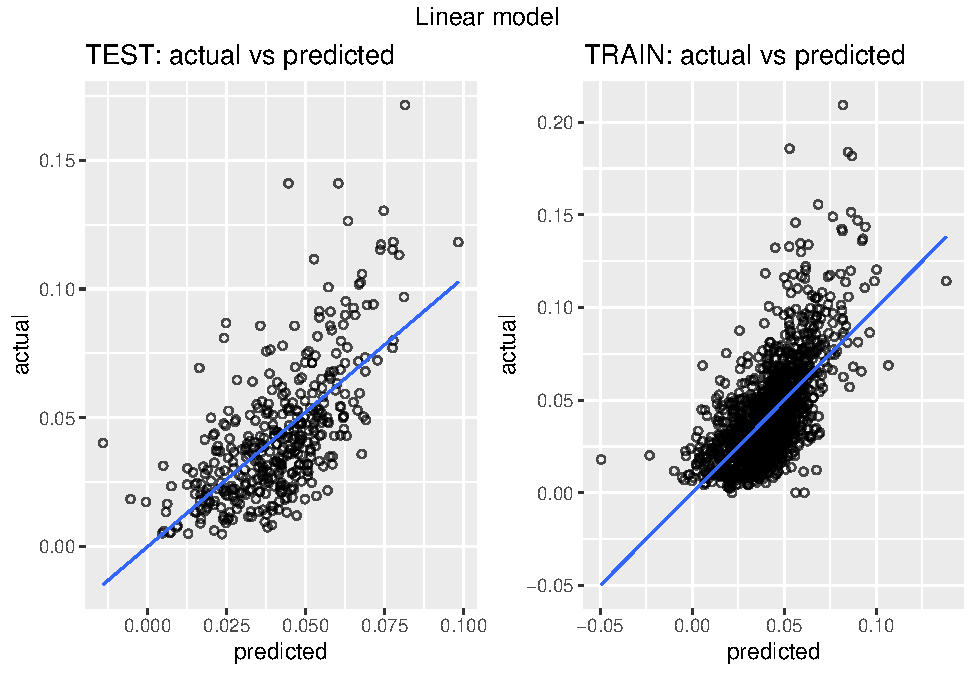
\includegraphics{Lin_Mod_Clus_Anal_files/figure-latex/unnamed-chunk-22-1.pdf}

\begin{Shaded}
\begin{Highlighting}[]
\CommentTok{\# qplot(d.train$GA\_share, predict.lm(lm1, d.train), colour = d.train$language)}
\CommentTok{\# plot(lm1)}
\end{Highlighting}
\end{Shaded}

Now the same for the GLM:

\begin{Shaded}
\begin{Highlighting}[]
\NormalTok{glmte }\OtherTok{\textless{}{-}} \FunctionTok{ggplot}\NormalTok{(d.test, }\FunctionTok{aes}\NormalTok{(}\AttributeTok{y=}\NormalTok{GA\_share ,}\AttributeTok{x=}\FunctionTok{predict}\NormalTok{(glmodel1, d.test, }\AttributeTok{type=}\StringTok{"response"}\NormalTok{))) }\SpecialCharTok{+}
  \FunctionTok{labs}\NormalTok{(}\AttributeTok{y=} \StringTok{"actual"}\NormalTok{, }\AttributeTok{x =} \StringTok{"predicted"}\NormalTok{) }\SpecialCharTok{+} \FunctionTok{ggtitle}\NormalTok{(}\StringTok{"TEST: actual vs predicted"}\NormalTok{) }\SpecialCharTok{+} 
  \FunctionTok{geom\_point}\NormalTok{(}\AttributeTok{shape =} \DecValTok{1}\NormalTok{, }\AttributeTok{alpha =} \FloatTok{0.7}\NormalTok{)}

\NormalTok{glmtr }\OtherTok{\textless{}{-}} \FunctionTok{ggplot}\NormalTok{(d.train,}\FunctionTok{aes}\NormalTok{(}\AttributeTok{y=}\NormalTok{GA\_share, }\AttributeTok{x=}\FunctionTok{predict}\NormalTok{(glmodel1, d.train, }\AttributeTok{type=}\StringTok{"response"}\NormalTok{))) }\SpecialCharTok{+}
  \FunctionTok{labs}\NormalTok{(}\AttributeTok{y=} \StringTok{"actual"}\NormalTok{, }\AttributeTok{x =} \StringTok{"predicted"}\NormalTok{) }\SpecialCharTok{+} \FunctionTok{ggtitle}\NormalTok{(}\StringTok{"TRAIN: actual vs predicted"}\NormalTok{) }\SpecialCharTok{+} 
  \FunctionTok{geom\_point}\NormalTok{(}\AttributeTok{shape =} \DecValTok{1}\NormalTok{, }\AttributeTok{alpha =} \FloatTok{0.7}\NormalTok{)}

\NormalTok{gridExtra}\SpecialCharTok{::}\FunctionTok{grid.arrange}\NormalTok{(}\AttributeTok{nrow =} \DecValTok{1}\NormalTok{, }\AttributeTok{ncol =} \DecValTok{2}\NormalTok{, }
\NormalTok{                        glmte }\SpecialCharTok{+} \FunctionTok{stat\_smooth}\NormalTok{(}\AttributeTok{size=}\FloatTok{0.5}\NormalTok{, }\AttributeTok{method=}\StringTok{"glm"}\NormalTok{,}\AttributeTok{se=}\ConstantTok{FALSE}\NormalTok{),}
\NormalTok{                        glmtr }\SpecialCharTok{+} \FunctionTok{stat\_smooth}\NormalTok{(}\AttributeTok{size=}\FloatTok{0.5}\NormalTok{, }\AttributeTok{method=}\StringTok{"glm"}\NormalTok{,}\AttributeTok{se=}\ConstantTok{FALSE}\NormalTok{),}
                        \AttributeTok{top=}\StringTok{"GLM Quasibinomial model"}\NormalTok{)}
\end{Highlighting}
\end{Shaded}

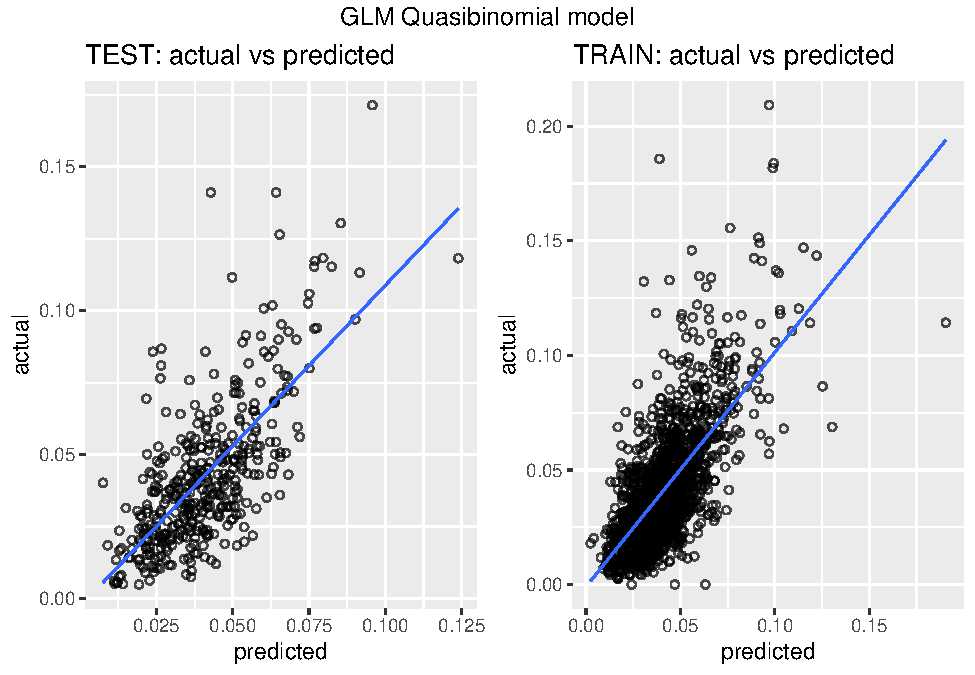
\includegraphics{Lin_Mod_Clus_Anal_files/figure-latex/unnamed-chunk-23-1.pdf}

\begin{Shaded}
\begin{Highlighting}[]
\CommentTok{\# qplot(d.train$GA\_share, predict(glmodel1, d.train, type="response"), colour = d.train$language)}
\CommentTok{\# plot(glmodel1)}
\end{Highlighting}
\end{Shaded}

\hypertarget{evaluation-results}{%
\subsubsection{Evaluation results}\label{evaluation-results}}

Now the comparison of the RMSE and Rsquare values:

First the values for the linear model, which takes all variables into
account:

\begin{Shaded}
\begin{Highlighting}[]
\NormalTok{lm0.eval.train }\OtherTok{\textless{}{-}} \FunctionTok{eval\_results}\NormalTok{(d.train}\SpecialCharTok{$}\NormalTok{GA\_share, }\FunctionTok{predict.lm}\NormalTok{(lm0, d.train))}
\NormalTok{lm0.eval.test }\OtherTok{\textless{}{-}} \FunctionTok{eval\_results}\NormalTok{(d.test}\SpecialCharTok{$}\NormalTok{GA\_share, }\FunctionTok{predict.lm}\NormalTok{(lm0, d.test))}

\FunctionTok{writeLines}\NormalTok{(}\FunctionTok{paste}\NormalTok{(}\StringTok{"Lm0: RMSE train: "}\NormalTok{, }\FunctionTok{round}\NormalTok{(}\FunctionTok{exp}\NormalTok{(lm0.eval.train}\SpecialCharTok{$}\NormalTok{RMSE), }\DecValTok{3}\NormalTok{),}
                 \StringTok{"}\SpecialCharTok{\textbackslash{}n}\StringTok{Lm0: Rsquare train: "}\NormalTok{,}\FunctionTok{round}\NormalTok{(lm0.eval.train}\SpecialCharTok{$}\NormalTok{Rsquare, }\DecValTok{3}\NormalTok{),}
                 \StringTok{"}\SpecialCharTok{\textbackslash{}n}\StringTok{Lm0: RMSE test: "}\NormalTok{, }\FunctionTok{round}\NormalTok{(}\FunctionTok{exp}\NormalTok{(lm0.eval.test}\SpecialCharTok{$}\NormalTok{RMSE), }\DecValTok{3}\NormalTok{),}
                 \StringTok{"}\SpecialCharTok{\textbackslash{}n}\StringTok{Lm0: Rsquare test: "}\NormalTok{, }\FunctionTok{round}\NormalTok{(lm0.eval.test}\SpecialCharTok{$}\NormalTok{Rsquare, }\DecValTok{3}\NormalTok{)))}
\end{Highlighting}
\end{Shaded}

\begin{verbatim}
## Lm0: RMSE train:  1.019 
## Lm0: Rsquare train:  0.47 
## Lm0: RMSE test:  1.019 
## Lm0: Rsquare test:  0.475
\end{verbatim}

\begin{Shaded}
\begin{Highlighting}[]
\CommentTok{\# qplot(d.train$GA\_share, predict.lm(lm0, d.train), colour = d.train$language)}
\end{Highlighting}
\end{Shaded}

Second, the values for the linear model, which takes only selected
variables into account:

\begin{Shaded}
\begin{Highlighting}[]
\NormalTok{lm1.eval.train }\OtherTok{\textless{}{-}} \FunctionTok{eval\_results}\NormalTok{(d.train}\SpecialCharTok{$}\NormalTok{GA\_share, }\FunctionTok{predict.lm}\NormalTok{(lm1, d.train)) }
\NormalTok{lm1.eval.test }\OtherTok{\textless{}{-}} \FunctionTok{eval\_results}\NormalTok{(d.test}\SpecialCharTok{$}\NormalTok{GA\_share, }\FunctionTok{predict.lm}\NormalTok{(lm1, d.test))}

\FunctionTok{writeLines}\NormalTok{(}\FunctionTok{paste}\NormalTok{(}\StringTok{"Lm1: RMSE train: "}\NormalTok{, }\FunctionTok{round}\NormalTok{(}\FunctionTok{exp}\NormalTok{(lm1.eval.train}\SpecialCharTok{$}\NormalTok{RMSE), }\DecValTok{3}\NormalTok{), }
                 \StringTok{"}\SpecialCharTok{\textbackslash{}n}\StringTok{Lm1: Rsquare train: "}\NormalTok{,}\FunctionTok{round}\NormalTok{(lm1.eval.train}\SpecialCharTok{$}\NormalTok{Rsquare, }\DecValTok{3}\NormalTok{), }
                 \StringTok{"}\SpecialCharTok{\textbackslash{}n}\StringTok{Lm1: RMSE test: "}\NormalTok{, }\FunctionTok{round}\NormalTok{(}\FunctionTok{exp}\NormalTok{(lm1.eval.test}\SpecialCharTok{$}\NormalTok{RMSE), }\DecValTok{3}\NormalTok{), }
                 \StringTok{"}\SpecialCharTok{\textbackslash{}n}\StringTok{Lm1: Rsquare test: "}\NormalTok{, }\FunctionTok{round}\NormalTok{(lm1.eval.test}\SpecialCharTok{$}\NormalTok{Rsquare, }\DecValTok{3}\NormalTok{)))}
\end{Highlighting}
\end{Shaded}

\begin{verbatim}
## Lm1: RMSE train:  1.019 
## Lm1: Rsquare train:  0.467 
## Lm1: RMSE test:  1.019 
## Lm1: Rsquare test:  0.471
\end{verbatim}

And second the values for the GLM:

\begin{Shaded}
\begin{Highlighting}[]
\NormalTok{glmodel0.eval.train }\OtherTok{\textless{}{-}} \FunctionTok{eval\_results}\NormalTok{(d.train[,}\DecValTok{4}\SpecialCharTok{:}\DecValTok{45}\NormalTok{]}\SpecialCharTok{$}\NormalTok{GA\_share, }\FunctionTok{predict}\NormalTok{(glmodel0, d.train[,}\DecValTok{4}\SpecialCharTok{:}\DecValTok{45}\NormalTok{], }\AttributeTok{type=}\StringTok{"response"}\NormalTok{)) }
\NormalTok{glmodel0.eval.test }\OtherTok{\textless{}{-}} \FunctionTok{eval\_results}\NormalTok{(d.test[,}\DecValTok{4}\SpecialCharTok{:}\DecValTok{45}\NormalTok{]}\SpecialCharTok{$}\NormalTok{GA\_share, }\FunctionTok{predict}\NormalTok{(glmodel0, d.test[,}\DecValTok{4}\SpecialCharTok{:}\DecValTok{45}\NormalTok{], }\AttributeTok{type=}\StringTok{"response"}\NormalTok{))}

\FunctionTok{writeLines}\NormalTok{(}\FunctionTok{paste}\NormalTok{(}\StringTok{"GLM0: RMSE train: "}\NormalTok{, }\FunctionTok{round}\NormalTok{(}\FunctionTok{exp}\NormalTok{(glmodel0.eval.train}\SpecialCharTok{$}\NormalTok{RMSE), }\DecValTok{3}\NormalTok{), }
                 \StringTok{"}\SpecialCharTok{\textbackslash{}n}\StringTok{GLM0: Rsquare train: "}\NormalTok{,}\FunctionTok{round}\NormalTok{(glmodel0.eval.train}\SpecialCharTok{$}\NormalTok{Rsquare, }\DecValTok{3}\NormalTok{),}
                 \StringTok{"}\SpecialCharTok{\textbackslash{}n}\StringTok{GLM0: RMSE test: "}\NormalTok{, }\FunctionTok{round}\NormalTok{(}\FunctionTok{exp}\NormalTok{(glmodel0.eval.test}\SpecialCharTok{$}\NormalTok{RMSE), }\DecValTok{3}\NormalTok{), }
                 \StringTok{"}\SpecialCharTok{\textbackslash{}n}\StringTok{GLM0: Rsquare test: "}\NormalTok{, }\FunctionTok{round}\NormalTok{(glmodel0.eval.test}\SpecialCharTok{$}\NormalTok{Rsquare, }\DecValTok{3}\NormalTok{)))}
\end{Highlighting}
\end{Shaded}

\begin{verbatim}
## GLM0: RMSE train:  1.018 
## GLM0: Rsquare train:  0.519 
## GLM0: RMSE test:  1.018 
## GLM0: Rsquare test:  0.53
\end{verbatim}

\begin{Shaded}
\begin{Highlighting}[]
\NormalTok{glmodel1.eval.train }\OtherTok{\textless{}{-}} \FunctionTok{eval\_results}\NormalTok{(d.train[,}\DecValTok{4}\SpecialCharTok{:}\DecValTok{45}\NormalTok{]}\SpecialCharTok{$}\NormalTok{GA\_share, }\FunctionTok{predict}\NormalTok{(glmodel1, d.train[,}\DecValTok{4}\SpecialCharTok{:}\DecValTok{45}\NormalTok{], }\AttributeTok{type=}\StringTok{"response"}\NormalTok{)) }
\NormalTok{glmodel1.eval.test }\OtherTok{\textless{}{-}} \FunctionTok{eval\_results}\NormalTok{(d.test[,}\DecValTok{4}\SpecialCharTok{:}\DecValTok{45}\NormalTok{]}\SpecialCharTok{$}\NormalTok{GA\_share, }\FunctionTok{predict}\NormalTok{(glmodel1, d.test[,}\DecValTok{4}\SpecialCharTok{:}\DecValTok{45}\NormalTok{], }\AttributeTok{type=}\StringTok{"response"}\NormalTok{))}

\FunctionTok{writeLines}\NormalTok{(}\FunctionTok{paste}\NormalTok{(}\StringTok{"GLM1: RMSE train: "}\NormalTok{, }\FunctionTok{round}\NormalTok{(}\FunctionTok{exp}\NormalTok{(glmodel1.eval.train}\SpecialCharTok{$}\NormalTok{RMSE), }\DecValTok{3}\NormalTok{), }
                 \StringTok{"}\SpecialCharTok{\textbackslash{}n}\StringTok{GLM1: Rsquare train: "}\NormalTok{,}\FunctionTok{round}\NormalTok{(glmodel1.eval.train}\SpecialCharTok{$}\NormalTok{Rsquare, }\DecValTok{3}\NormalTok{),}
                 \StringTok{"}\SpecialCharTok{\textbackslash{}n}\StringTok{GLM1: RMSE test: "}\NormalTok{, }\FunctionTok{round}\NormalTok{(}\FunctionTok{exp}\NormalTok{(glmodel1.eval.test}\SpecialCharTok{$}\NormalTok{RMSE), }\DecValTok{3}\NormalTok{), }
                 \StringTok{"}\SpecialCharTok{\textbackslash{}n}\StringTok{GLM1: Rsquare test: "}\NormalTok{, }\FunctionTok{round}\NormalTok{(glmodel1.eval.test}\SpecialCharTok{$}\NormalTok{Rsquare, }\DecValTok{3}\NormalTok{)))}
\end{Highlighting}
\end{Shaded}

\begin{verbatim}
## GLM1: RMSE train:  1.018 
## GLM1: Rsquare train:  0.515 
## GLM1: RMSE test:  1.018 
## GLM1: Rsquare test:  0.523
\end{verbatim}

\hypertarget{cluster-analysis}{%
\section{CLUSTER ANALYSIS}\label{cluster-analysis}}

The best model of the different approaches will result in the highest
accuracy and a corresponding list of parameters which are relevant and
should be focussed on in the cluster analysis. Many, diverse communities
can make it difficult to find easily separable clusters. Therefore, the
first step of the cluster analysis is the reduction of the data to the
cantonal level. For this purpose, a separate table must be created with
a similar procedure as described in chapter 5.2.2, with the shares
calculated on this new level of aggregation. Different options of
cluster methods will be integrated in the analysis. I will use an
agglomerative clustering model to start, which does not need a
pre-defined number of clusters (Ward, 1963). This is an advantage,
especially because it is hard to estimate in advance what number of
groups will be useful at the end. Alternative models would be a k-means
clustering (partitioning method) with a given number of clusters
(MacQueen, 1967), a Generalized Mixture Model (GMM) which uses
statistical models and is not based simply on a distance measure
(Rasmussen, 1999), or even a density-based clustering like DBSCAN which
assigns points to clusters based on densities in the data, returning
also outliers (Ester et al., 1996).

\begin{Shaded}
\begin{Highlighting}[]
\FunctionTok{summary}\NormalTok{(cars)}
\end{Highlighting}
\end{Shaded}

\begin{verbatim}
##      speed           dist       
##  Min.   : 4.0   Min.   :  2.00  
##  1st Qu.:12.0   1st Qu.: 26.00  
##  Median :15.0   Median : 36.00  
##  Mean   :15.4   Mean   : 42.98  
##  3rd Qu.:19.0   3rd Qu.: 56.00  
##  Max.   :25.0   Max.   :120.00
\end{verbatim}

\hypertarget{including-plots}{%
\subsection{Including Plots}\label{including-plots}}

You can also embed plots, for example:

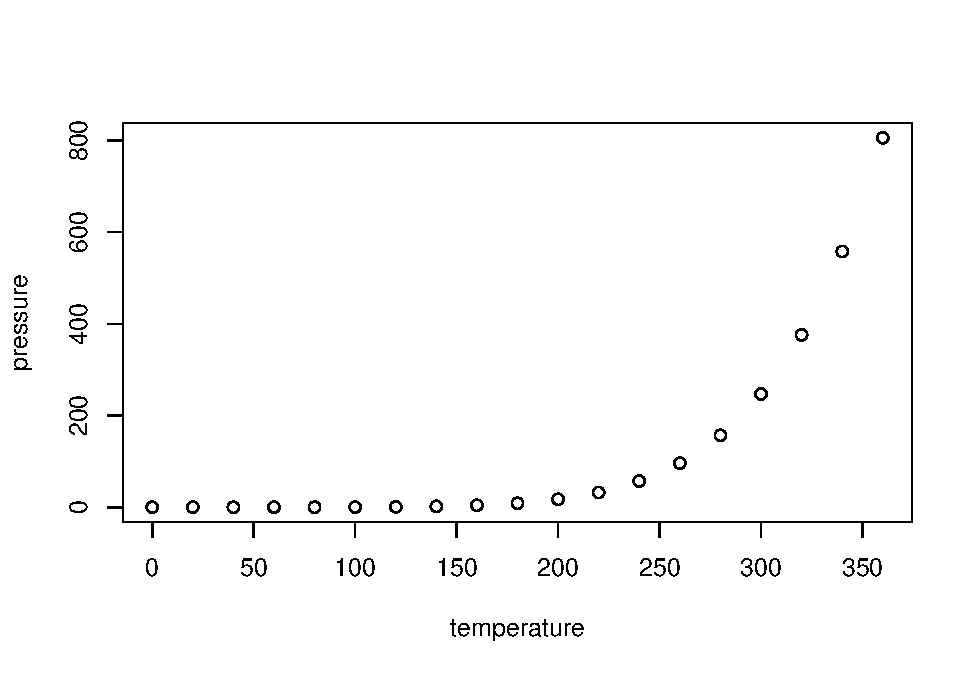
\includegraphics{Lin_Mod_Clus_Anal_files/figure-latex/pressure-1.pdf}

Note that the \texttt{echo\ =\ FALSE} parameter was added to the code
chunk to prevent printing of the R code that generated the plot.

\end{document}
